\section{Introduction}

As a default the \D integration algorithms\index{algorithm} are
based on the Velocity Verlet\index{algorithm!Verlet} (VV) scheme,
which is both simple and time reversible \cite{allen-89a}.  It
generates trajectories in the microcanonical (NVE) ensemble in
which the total energy (kinetic plus potential) is conserved.  If
this property drifts or fluctuates excessively in the course of a
simulation it indicates that the timestep is too large or the
potential cutoffs too small (relative r.m.s. fluctuations in the
total energy of $10^{-5}$ are typical with this algorithm).

The VV algorithm has two stages (VV1 and VV2). At the first stage
it requires values of position ($\vek{r}$), velocity ($\vek{v}$)
and force ($\vek{f}$) at time $t$.  The first stage is to advance
the velocities to $t+(1/2)\Delta t$ by integration of the force
and then to advance the positions to a full step $t+\Delta t$
using the new half-step velocities:
\begin{enumerate}
\item VV1:
\begin{equation}
\vek{v}(t + {1 \over 2} \Delta t) \leftarrow \vek{v}(t) + {\Delta t \over 2} \;
{\vek{f}(t) \over m}~~,
\end{equation}
where $m$ is the mass of a site and $\Delta t$ is the timestep
\begin{equation}
\vek{r}(t + \Delta t) \leftarrow \vek{r}(t) + \Delta t \;
\vek{v}(t + {1 \over 2}\Delta t)
\end{equation}
\item FF:
\newline Between the first and the second stage a recalculation of the force
at time $t+\Delta t$ is required since the positions have changed
\begin{equation}
\vek{f}(t + \Delta t) \leftarrow \vek{f}(t)
\end{equation}
\item VV2:
\newline In the second stage the half-step velocities
are advanced to to a full step using the new force
\begin{equation}
\vek{v}(t + \Delta t) \leftarrow  \vek{v}(t + {1 \over 2} \Delta t) +
{\Delta t \over 2} \; {\vek{f}(t + \Delta t) \over m}
\end{equation}
\end{enumerate}

\D also offers integration algorithms based on the leapfrog Verlet
(LFV) scheme \cite{allen-89a}.  Although LFV scheme is somewhat
simpler and numerically faster than the VV scheme, it is not time
reversible and does not offer the numerical stability the VV scheme
does.  Furthermore, all kinetic related properties have approximate
estimators due to the half a step out of phase between velocity and position.

The LFV algorithm is one staged.  It requires values of position
($\vek{r}$) and force ($\vek{f}$) at time $t$ and  velocity
($\vek{v}$) at half a timestep behind: $t-(1/2)\Delta t$.  Firstly,
the forces are recalculated afresh at time $t$ (from time
$t-\Delta t$) since the positions have changed from the last step:
\begin{enumerate}
\item FF:
\begin{equation}
\vek{f}(t) \leftarrow \vek{f}(t - \Delta t)~~,
\end{equation}
where $\Delta t$ is the timestep
\item LFV:
\newline The velocities are advanced by a timestep to
$t+(1/2)\Delta t$ by integration of the new force
\begin{equation}
\vek{v}(t + {1 \over 2} \Delta t) \leftarrow \vek{v}(t - {1 \over 2} \Delta t) +
\Delta t \; {\vek{f}(t) \over m}~~,
\end{equation}
where $m$ is the mass of a site, and then the positions are
advanced to a full step $t+\Delta t$ using the new half-step
velocities
\begin{equation}
\vek{r}(t + \Delta t) \leftarrow \vek{r}(t) + \Delta t \;
\vek{v}(t + {1 \over 2}\Delta t)
\end{equation}
\end{enumerate}
Molecular dynamics simulations normally require properties that
depend on position and velocity {\em at the same time} (such as
the sum of potential and kinetic energy).  The velocity at time
$t$ is obtained from the average of the velocities half a timestep
either side of timestep $t$:
\begin{equation}
\vek{v}(t) \leftarrow {1 \over 2} \left[ \vek{v}(t - {1 \over 2} \Delta t) +
\vek{v}(t + {1 \over 2} \Delta t) \right]~~.
\end{equation}

The instantaneous kinetic energy, for example, can then be
obtained from the atomic velocities as
\begin{equation}
E_{kin}(t) = {1 \over 2} \sum_{1}^{\cal N} m_{i} v_{i}^{2}(t)~~, \label{ekin}
\end{equation}
and assuming the system has no net momentum the instantaneous
temperature is
\begin{equation}
{\cal T}(t) = \frac{2}{k_{B} f} E_{kin}(t)~~, \label{tinst}
\end{equation}
where $i$ labels particles (that can be free atoms or
rigid bodies\index{rigid body}), ${\cal N}$ the number of particles
(free atoms and rigid bodies\index{rigid body}) in
the system, $k_{B}$ the Boltzmann's constant and $f$ the number of
degrees of freedom in the system.
\begin{equation}
f = 3{\cal N} - 3{\cal N}_{frozen} - 3{\cal N}_{shells} -
{\cal N}_{constraints} - 3 - p~~. \label{freedom}
\end{equation}
Here ${\cal N}_{frozen}$ indicates the number of frozen atoms in
the system, ${\cal N}_{shells}$ number of core-shell units and
${\cal N}_{constraints}$ number of bond and PMF constraints.
Three degrees of freedom are subtracted for the centre of mass
zero net momentum (which we impose) and $p$ is zero for periodic
or three for non-periodic systems, where it accounts for fixing
angular momentum about origin (which we impose).

In the case of rigid bodies\index{rigid body} (see Section~\ref{rigid})
the first part of equation~(\ref{freedom})
\begin{equation}
f\prime = 3{\cal N} - 3{\cal N}_{frozen}
\end{equation}
splits into
\begin{equation}
f\prime = \left( 3{\cal N}^{FP} - 3{\cal N}^{FP}_{frozen} \right) +
          \left( 3{\cal N}^{RB {\bf (tra)}} - 3{\cal N}^{RB {\bf (tra)}}_{frozen} \right) +
          \left( 3{\cal N}^{RB {\bf (rot)}} - 3{\cal N}^{RB {\bf (rot)}}_{frozen} \right)
\end{equation}
or
\begin{equation}
f\prime = f^{FP} + f^{RB {\bf (tra)}} + f^{RB {\bf (rot)}}~~.
\end{equation}
Here FP stands for a free particle, i.e. a particle not
participating in the constitution of a rigid body, and RB for a
rigid body.  In general a rigid body has 3 translational (${\bf tra}$)
degrees of freedom, corresponding to its centre of mass being allowed
to move in the 3 general direction of space, and 3 rotational
(${\bf rot}$), corresponding to the RB being allowed to rotate around
the 3 general axis in space.  It is not far removed to see that for
a not fully frozen rigid body one must assign 0 translational degrees
of freedom but depending on the "frozenness" of the RB one may assign
1 rotational degrees of freedom when all the frozen sites are in line
(i.e. rotation around one axis only) or 3 when just one site is frozen.

The routines {\sc nve\_0\_vv} and {\sc nve\_0\_lfv} implement the
Verlet\index{algorithm!Verlet} algorithm in velocity and leapfrog
flavours respectively for free particles and calculate the
instantaneous temperature.  Whereas the routines {\sc nve\_1\_vv} and
{\sc nve\_1\_lfv} implement the same for systems also containing
rigid bodies.  The conserved quantity is the total energy of the system
\begin{equation}
{\cal H}_{\rm NVE} = U + E_{kin}~~,
\end{equation}
where $U$ is the potential energy of the system and $E_{kin}$ the
kinetic energy at time $t$.

The full selection of integration algorithms, indicating both VV and
LFV cast integration, within \D is as follows:

\begin{tabbing}
XXXXXXXXXXXXX\=XXXXXXXXXX\=XXXXXXXXXXXXXXXXXXXXXXXXXXXXXXXXXXXXXXXXXXXXXXXX\kill\\
{\sc nve\_0\_vv}      \> {\sc nve\_0\_lfv}  \> Constant E algorithm\index{ensemble!NVE} \\
{\sc nve\_1\_vv}      \> {\sc nve\_1\_lfv}  \> The same as the above but also incorporating RB integration \\
{\sc dpd\_thermostat} \> N/A            \> Constant T algorithm\index{ensemble!DPD NVT} (DPD \cite{shardlow-03a}) \\
{\sc nvt\_e0\_vv}     \> {\sc nvt\_e0\_lfv} \> Constant $E_{kin}$ algorithm\index{ensemble!Evans NVT} (Evans \cite{evans-84a}) \\
{\sc nvt\_e1\_vv}     \> {\sc nvt\_e1\_lfv} \> The same as the above but also incorporating RB integration \\
{\sc nvt\_l0\_vv}     \> {\sc nvt\_l0\_lfv} \> Constant T algorithm\index{ensemble!Langevin NVT} (Langevin \cite{adelman-76a}) \\
{\sc nvt\_l1\_vv}     \> {\sc nvt\_l1\_lfv} \> The same as the above but also incorporating RB integration \\
{\sc nvt\_a0\_vv}     \> {\sc nvt\_a0\_lfv} \> Constant T algorithm\index{ensemble!Andersen NVT} (Andersen \cite{andersen-79a}) \\
{\sc nvt\_a1\_vv}     \> {\sc nvt\_a1\_lfv} \> The same as the above but also incorporating RB integration \\
{\sc nvt\_b0\_vv}     \> {\sc nvt\_b0\_lfv} \> Constant T algorithm\index{ensemble!Berendsen NVT} (Berendsen \cite{berendsen-84a}) \\
{\sc nvt\_b1\_vv}     \> {\sc nvt\_b1\_lfv} \> The same as the above but also incorporating RB integration \\
{\sc nvt\_h0\_vv}     \> {\sc nvt\_h0\_lfv} \> Constant T algorithm\index{ensemble!Nos\'{e}-Hoover NVT} (Hoover \cite{hoover-85a}) \\
{\sc nvt\_h1\_vv}     \> {\sc nvt\_h1\_lfv} \> The same as the above but also incorporating RB integration \\
{\sc nvt\_g0\_vv}     \> {\sc nvt\_g0\_lfv} \> Constant T algorithm\index{ensemble!Gentle Stochastic NVT} (GST \cite{leimkuhler-09a}) \\
{\sc nvt\_g1\_vv}     \> {\sc nvt\_g1\_lfv} \> The same as the above but also incorporating RB integration \\
{\sc npt\_l0\_vv}     \> {\sc npt\_l0\_lfv} \> Constant T,P algorithm\index{ensemble!Langevin NPT} (Langevin \cite{quigley-04a}) \\
{\sc npt\_l1\_vv}     \> {\sc npt\_l1\_lfv} \> The same as the above but also incorporating RB integration \\
{\sc npt\_b0\_vv}     \> {\sc npt\_b0\_lfv} \> Constant T,P algorithm\index{ensemble!Berendsen NPT} (Berendsen \cite{berendsen-84a}) \\
{\sc npt\_b1\_vv}     \> {\sc npt\_b1\_lfv} \> The same as the above but also incorporating RB integration \\
{\sc npt\_h0\_vv}     \> {\sc npt\_h0\_lfv} \> Constant T,P algorithm\index{ensemble!Nos\'{e}-Hoover NPT} (Hoover \cite{hoover-85a}) \\
{\sc npt\_h1\_vv}     \> {\sc npt\_h1\_lfv} \> The same as the above but also incorporating RB integration \\
{\sc npt\_m0\_vv}     \> {\sc npt\_m0\_lfv} \> Constant T,P algorithm\index{ensemble!Martyna-Tuckerman-Klein NPT} (Martyna-Tuckerman-Klein \cite{martyna-96a}) \\
{\sc npt\_m1\_vv}     \> {\sc npt\_m1\_lfv} \> The same as the above but also incorporating RB integration \\
{\sc npt\_l0\_vv}     \> {\sc npt\_l0\_lfv} \> Constant T,$\mat{\sigma}$ algorithm\index{ensemble!Langevin N$\sigma$T} (Langevin \cite{quigley-04a}) \\
{\sc npt\_l1\_vv}     \> {\sc npt\_l1\_lfv} \> The same as the above but also incorporating RB integration \\
{\sc nst\_b0\_vv}     \> {\sc nst\_b0\_lfv} \> Constant T,$\mat{\sigma}$ algorithm\index{ensemble!Berendsen N$\sigma$T} (Berendsen \cite{berendsen-84a}) \\
{\sc nst\_b1\_vv}     \> {\sc nst\_b1\_lfv} \> The same as the above but also incorporating RB integration \\
{\sc nst\_h0\_vv}     \> {\sc nst\_h0\_lfv} \> Constant T,$\mat{\sigma}$ algorithm\index{ensemble!Nos\'{e}-Hoover N$\sigma$T} (Hoover \cite{hoover-85a}) \\
{\sc nst\_h1\_vv}     \> {\sc nst\_h1\_lfv} \> The same as the above but also incorporating RB integration \\
{\sc nst\_m0\_vv}     \> {\sc nst\_m0\_lfv} \> Constant T,$\mat{\sigma}$ algorithm\index{ensemble!Martyna-Tuckerman-Klein N$\sigma$T} (Martyna-Tuckerman-Klein \cite{martyna-96a}) \\
{\sc nst\_m0\_vv}     \> {\sc nst\_m0\_lfv} \> The same as the above but also incorporating RB integration
\end{tabbing}

It is worth noting that the last four ensembles are also optionally
available in an extended from to constant normal pressure and
constant surface area, NP$_{n}$AT, or constant surface tension,
NP$_{n}\gamma$T \cite{ikeguchi-04a}.

\section{Bond Constraints}
\label{shake-rattle}

The SHAKE algorithm \index{algorithm!SHAKE} for bond constraints
was devised by Ryckaert {\em et al.} \cite{ryckaert-77a} and is
widely used in molecular simulation.  It is a two stage algorithm
based on the leapfrog Verlet\index{algorithm!Verlet} integration
scheme \cite{allen-89a}.  In the first stage the LFV algorithm
calculates the motion of the atoms in the system assuming a
complete absence of the rigid bond\index{rigid bond|see{constraints,bond}}
forces. The positions of the atoms at the end of this stage
do not conserve the distance constraint required by the
rigid bond\index{constraints!bond} and a correction is necessary.
In the second stage the deviation in the length of a given
rigid bond\index{constraints!bond} is used retrospectively to
compute the constraint force needed to conserve the bondlength.
It is relatively simple to show that the constraint force has the form:
\begin{equation}
\vek{G}_{ij} \approx\ {1 \over 2} {\mu_{ij} \over \Delta t^{2}} \;
{(d_{ij}^{2} - d_{ij}'^{2}) \over \vek{d}_{ij}^{o} \cdot
\vek{d}_{ij}'} \; \vek{d}_{ij}^{o}~~, \label{g12}
\end{equation}
where: $\mu_{ij}$ is the reduced mass of the two atoms connected
by the bond; $\vek{d}_{ij}^{o}$ and $\vek{d}_{ij}'$ are the
original and intermediate bond vectors; $d_{ij}$ is the
constrained bondlength; and $\Delta t$ is the
Verlet\index{algorithm!Verlet} integration time step.  It should
be noted that this formula is an approximation only.

\begin{figure}[htbp]
\begin{center}
\vskip 1ex
\centerline{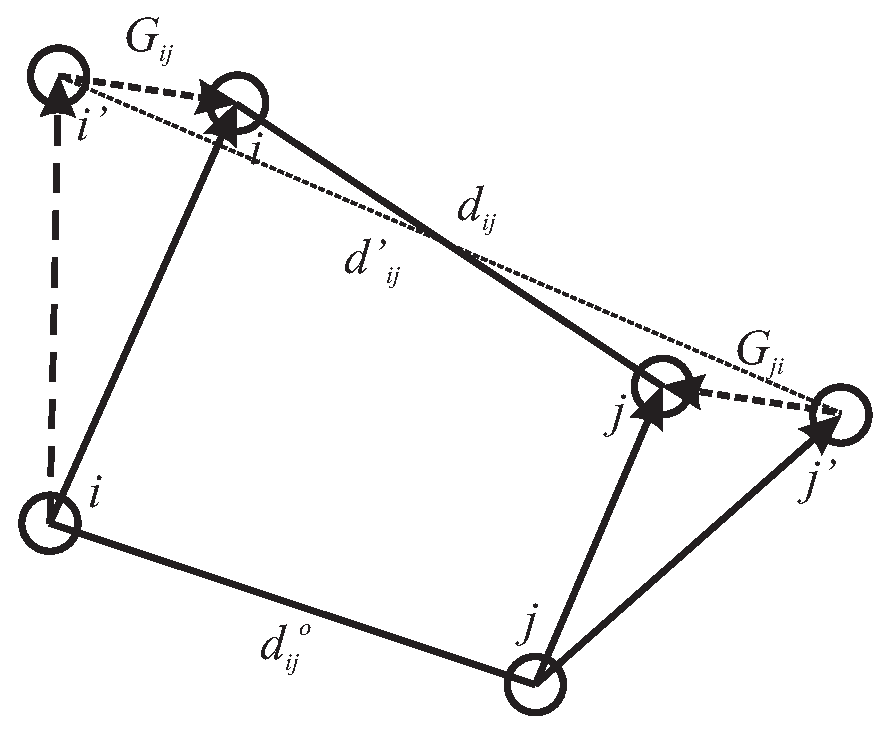
\includegraphics[height=8.0cm]{shake.eps}}
\caption[The SHAKE (RATTLE\_VV1) schematics and associated vectors]
{The SHAKE (RATTLE\_VV1) schematics and associated vectors.  The
algorithm calculates the constraint force $\vek{G}_{ij}=-\vek{G}_{ji}$
that conserves the bondlength $d_{ij}$ between atoms $i$ and $j$,
following the initial movement to positions $i\prime$ and $j\prime$
under the unconstrained forces $\vek{F}_{i}$ and $\vek{F}_{j}$ and
velocities $\vek{v}_{i}$ and $\vek{v}_{j}$.}
%\vskip 1ex
\end{center}
\end{figure}

The RATTLE algorithm \index{algorithm!RATTLE} was devised by
Andersen \cite{andersen-83a} and it fits within the concept of the
Velocity Verlet\index{algorithm!Verlet} integration scheme.  It
consists of two parts RATTLE\_VV1 and RATTLE\_VV2 applied
respectively in stages one and two of Velocity
Verlet\index{algorithm!Verlet} algorithm.  RATTLE\_VV1 is similar to
the SHAKE algorithm as described above and handles the bond length
constraint.  However, due to the difference in the velocity update
between VV (VV1) and LFV schemes, the constraint force generated to
conserve the bondlength in RATTLE\_VV1 has the form as in
(\ref{g12}) but missing the factor of a half:
\begin{equation}
\vek{G}_{ij} \approx\ {\mu_{ij} \over \Delta t^{2}} \;
{(d_{ij}^{2} - d_{ij}'^{2}) \over \vek{d}_{ij}^{o} \cdot
\vek{d}_{ij}'} \; \vek{d}_{ij}^{o}~~. \label{g121}
\end{equation}
The constraint force in RATTLE\_VV2 imposes a new condition of
rigidity on constraint bonded atom velocities.  RATTLE\_VV2 is
also a two stage algorithm.  In the first stage, the VV2 algorithm
calculates the velocities of the atoms in the system assuming a
complete absence of the rigid bond\index{rigid bond|see{constraints,bond}}
forces (since forces have just been recalculated afresh after VV1).
The relative velocity of atom {i} with respect to atom {j}
(or vice versa) constituting the rigid bond {ij} may not be
perpendicular to the bond -  i.e. may have a non-zero component
along the bond. However, by the stricter definition of rigidity
this is is required to be zero as it will otherwise lead to a
change in the rigid bond length during the consequent timestepping.
In the second stage the deviation from zero of the scalar product
$\vek{d}_{ij}~\cdot~(\vek{v}_{j}~-~\vek{v}_{i})$ is used
retrospectively to compute the constraint force needed to keep the
bond rigid over the length of the timestep $\Delta t$.  It is
relatively simple to show that the constraint force has the form:
\begin{equation}
\vek{B}_{ij} \approx\ {\mu_{ij} \over \Delta t} \;
{\vek{d}_{ij} \cdot (\vek{v}_{j}-\vek{v}_{i}) \over
d_{ij}^{2}} \; \vek{d}_{ij}~~. \label{b12}
\end{equation}
The velocity corrections can therefore be written as
\begin{equation}
\vek{v}^{corr}_{i} = \Delta t \; {\vek{B}_{ij} \over m_{i}} =
{\mu_{ij} \over m_{i}} {\vek{d}_{ij} \cdot (\vek{v}_{j}-\vek{v}_{i}) \over
d_{ij}^{2}} \; \vek{d}_{ij}~~.
\end{equation}

For a system of simple diatomic molecules, computation of the
constraint force will, in principle, allow the correct atomic
positions to be calculated in one pass.  However, in the general
polyatomic case this correction is merely an interim adjustment, not
only because the above formula is approximate, but the successive
correction of other bonds in a molecule has the effect of perturbing
previously corrected bonds.  Either part of the RATTLE algorithm is
therefore iterative, with the correction cycle being repeated for
all bonds until: each has converged to the correct length, within a
given tolerance for RATTLE\_VV1 (SHAKE) and the relative bond
velocities are perpendicular to their respective bonds within a
given tolerance for RATTLE\_VV2 (RATTLE).  The tolerance may be of
the order $10^{-4}$~\AA~to $10^{-8}$~{\AA}~depending on the
precision desired.

The SHAKE procedure may be summarised as follows:
\begin{enumerate}
\item All atoms in the system are moved using the
LFV\index{algorithm!Verlet} algorithm, assuming an absence of
rigid bonds\index{constraints!bond} (constraint forces).  (This is
stage 1 of the SHAKE algorithm.)
\item The deviation in each bondlength is used to calculate the
corresponding constraint force, equation~(\ref{g12}), that (retrospectively)
`corrects' the bond length.
\item After the correction, equation~(\ref{g12}), has been applied to all
bonds, every bondlength is checked.  If the largest deviation found
exceeds the desired tolerance, the correction calculation is
repeated.
\item Steps 2 and 3 are repeated until all bondlengths
satisfy the convergence criterion (this iteration constitutes
stage 2 of the SHAKE algorithm).
\end{enumerate}

The RATTLE procedures may be summarised as follows:
\begin{enumerate}
\item RATTLE\index{algorithm!RATTLE} stage 1:
\begin{enumerate}
\item All atoms in the system are moved using the
VV\index{algorithm!Verlet} algorithm, assuming an absence of
rigid bonds\index{constraints!bond} (constraint forces).  (This is
stage 1 of the RATTLE\_VV1 algorithm.)
\item The deviation in each bondlength is used to calculate the
corresponding constraint force, equation~(\ref{g121}), that (retrospectively)
`corrects' the bond length.
\item After the correction, equation~(\ref{g121}), has been applied to all
bonds, every bondlength is checked.  If the largest deviation found
exceeds the desired tolerance, the correction calculation is
repeated.
\item Steps (b) and (c) are repeated until all
bondlengths satisfy the convergence criterion (this iteration
constitutes stage 2 of the RATTLE\_VV1 algorithm).
\end{enumerate}
\item Forces calculated afresh.
\item RATTLE\index{algorithm!Verlet} stage 2:
\begin{enumerate}
\item All atom velocities are updated to a full step, assuming an
absence of rigid bonds\index{constraints!bond}.  (This is stage 1
of the RATTLE\_VV2 algorithm.)
\item The deviation of $\vek{d}_{ij} \cdot (\vek{v}_{j}-\vek{d}_{i})$
in each bond is used to calculate the corresponding constraint
force that (retrospectively) `corrects' the bond velocities.
\item After the correction, equation~(\ref{b12}), has been applied to all
bonds, every bond velocity is checked against the above condition.  If the
largest deviation found exceeds the desired tolerance, the correction
calculation is repeated.
\item Steps (b) and (c) are repeated until all bonds satisfy the
convergence criterion (this iteration constitutes stage 2 of the
RATTLE\_VV2 algorithm).
\end{enumerate}
\end{enumerate}

The parallel version of the RATTLE algorithm, as implemented in
\D, is derived from the RD\_SHAKE\index{algorithm!SHAKE}
algorithm \cite{smith-94b} although its implementation in the
Domain Decomposition framework requires no {\em global merging}
operations and is consequently significantly more efficient.  The
routine {\sc constraints\_shake} is called to apply corrections to
the atomic positions and the routine {\sc constraints\_rattle} to
apply corrections to the atomic velocities of constrained particles.

It should be noted that the fully converged constraint forces
$G_{ij}$ make a contribution to the system virial and the stress
tensor\index{stress tensor}.

The contribution to be added to the atomic virial (for each
constrained bond) is
\begin{equation}
{\cal W} = -\vek{d}_{ij} \cdot \vek{G}_{ij}~~.
\end{equation}

The contribution to be added to the atomic stress
tensor\index{stress tensor} (for each constrained bond) is given
by
\begin{equation}
\sigma^{\alpha \beta} = d_{ij}^{\alpha} G_{ij}^{\beta}~~,
\end{equation}
where $\alpha$ and $\beta$ indicate the $x,y,z$ components. The
atomic stress tensor derived from the pair forces is symmetric.

\section{Potential of Mean Force (PMF)\index{constraints!PMF}
Constraints and the Evaluation of Free Energy}\label{pmf}

A generalization of bond constraints can be made to constrain
a system to some point along a reaction coordinate.  A simple
example of such a reaction coordinate would be the distance
between two ions in solution.  If a number of simulations are
conducted with the system constrained to different points along
the reaction coordinate then the mean constraint force may be
plotted as a function of reaction coordinate and the function
integrated to obtain the free energy for the overall process
\cite{mccammon-87a}.  The PMF constraint force, virial and
contributions to the stress tensor are obtained in a manner
analogous to that for a bond constraint (see previous section).
The only difference is that the constraint is now applied
between the centres of two groups which need not be atoms alone.
\D reports the PMF constraint virial, ${\cal W}_{PMF}$, for each
simulation.  Users can convert this to the PMF constraint force from
\begin{equation}
G_{PMF} = \frac {{\cal W}_{PMF}} {d_{PMF}}~~,
\end{equation}
where is $d_{PMF}$ the constraint distance between the two groups
used to define the reaction coordinate.

The routines {\sc pmf\_shake} and {\sc pmf\_rattle} are called to
apply corrections to the atomic positions and respectively the
atomic velocities of all particles constituting PMF units.

In presence of both bond constraints\index{constraints!bond} and
PMF constraints\index{constraints!PMF}.  The constraint procedures,
i.e. SHAKE or RATTLE, for both types of constraints are applied
iteratively in order bonds-PMFs until convergence of ${\cal W}_{PMF}$
reached.  The number of iteration cycles is limited by the same limit
as for the bond constraints' procedures (SHAKE/RATTLE).

\section{Thermostats}

The system may be coupled to a heat bath to ensure that the average
system temperature is maintained close to the requested temperature,
$T_{\rm ext}$.  When this is done the equations of motion are
modified and the system no longer samples the microcanonical
ensemble\index{ensemble!NVE}.  Instead trajectories in the canonical
(NVT) ensemble\index{ensemble!canonical}, or something close to it
are generated.  \D comes with seven different thermostats: Evans
(Gaussian constraints)\index{constraints!Gaussian} \cite{evans-84a},
Langevin \cite{adelman-76a,izaguirre-01a}, Andersen \cite{andersen-79a},
Berendsen \cite{berendsen-84a}, Nos\'e-Hoover (N-H) \cite{hoover-85a} and
the gentle stochastic thermostat (GST) \cite{leimkuhler-09a,samoletov-07a}
as well as Dissipative Particle Dynamics (DPD) method \index{DPD}
\cite{hoogerbrugge-92a,espanol-95a,groot-97a,shardlow-03a},  Of these,
only the Langevin, N-H, GST and DPD algorithms generate \emph{true}
trajectories in the canonical (NVT) ensemble.  The rest will produce
properties that typically differ from canonical averages by ${\cal O}(1/{\cal N})$
\cite{allen-89a} (where $\cal N$ is the number of particles in the system),
as the Evans algorithm generates trajectories in the (NVE$_{kin}$) ensemble.

\subsection{Evans Thermostat (Gaussian Constraints)}

Kinetic temperature can be made a constant of the equations of
motion by imposing an additional constraint on the system.  If one
writes the equations of motion as:
\begin{eqnarray}
{d \vek{r}(t) \over d t} &=& \vek{v}(t) \nonumber \\
{d \vek{v}(t) \over d t} &=& {\vek{f}(t) \over m} - \chi (t) \;
\vek{v}(t)~~,
\end{eqnarray}
the kinetic temperature constraint $\chi$ can be found as follows:
\begin{eqnarray}
\frac{d}{dt} {\cal T} &\propto& \frac{d}{dt} \left(\frac{1}{2}\sum_{i} m_{i} \vek{v}_{i}^{2} \right) =
\sum_{i} m_{i} \vek{v}_{i} \cdot \frac{d}{dt} \vek{v}_{i} = 0 \nonumber \\
& & \sum_{i} m_{i} \vek{v}_{i}(t) \cdot
\left\{ \frac{\vek{f}_{i}(t)}{m_{i}} - \chi (t) \; \vek{v}_{i}(t) \right\} = 0 \label{Evans} \\
\chi (t) &=& \frac {\sum_{i} \vek{v}_{i}(t) \cdot \vek{f}_{i}(t)} {\sum_{i} m_{i} \vek{v}_{i}^{2}(t)}~~, \nonumber
\end{eqnarray}
where $\cal T$ is the instantaneous temperature defined in equation~(\ref{tinst}).

The VV implementation of the Evans algorithm is straight forward.
The conventional VV1 and VV2 steps are carried out as before
the start of VV1 and after the end of VV2 there is an application of
thermal constraining.  This involves the calculation of $\chi (t)$
before the VV1 stage and $\chi (t+\Delta t)$ after the VV2 stage
with consecutive thermalisation on the unthermostated velocities
for half a timestep at each stage in the following manner:
\begin{enumerate}
\item Thermostat VV1
\begin{eqnarray}
\chi (t) &\leftarrow& \frac {\sum_{i} \vek{v}_{i}(t) \cdot \vek{f}_{i}(t)} {2~E_{kin}(t)} \nonumber \\
\vek{v}(t) &\leftarrow& \vek{v}(t)~\exp \left( -\chi (t) {\Delta t \over 2} \right)~~.
\end{eqnarray}
\item VV1:
\begin{eqnarray}
\vek{v}(t + {1 \over 2} \Delta t) &\leftarrow& \vek{v}(t) +
{\Delta t \over 2} \; {\vek{f}(t) \over m} \nonumber \\
\vek{r}(t + \Delta t) &\leftarrow& \vek{r}(t) + \Delta t \;
\vek{v}(t + {1 \over 2} \Delta t)
\end{eqnarray}
\item RATTLE\_VV1
\item FF:
\begin{equation}
\vek{f}(t + \Delta t) \leftarrow \vek{f}(t)
\end{equation}
\item VV2:
\begin{equation}
\vek{v}(t + \Delta t) \leftarrow \vek{v}(t + {1 \over 2} \Delta t) +
{\Delta t \over 2} \; \left[{\vek{f}(t + \Delta t) \over m} \right]
\end{equation}
\item RATTLE\_VV2
\item Thermostat VV2
\begin{eqnarray}
\chi (t + \Delta t) &\leftarrow& \frac {\sum_{i} \vek{v}_{i}(t +
\Delta t) \cdot \vek{f}_{i}(t + \Delta t)} {2~E_{kin}(t + \Delta t)} \nonumber \\
\vek{v}(t + \Delta t) &\leftarrow& \vek{v}(t + \Delta t)~
\exp \left( -\chi (t + \Delta t) {\Delta t \over 2} \right)~~.
\end{eqnarray}
\end{enumerate}
The algorithm is self-consistent and requires no iterations.

The LFV implementation of the Evans algorithm is iterative as an
initial estimate of $\chi (t)$ at full step is calculated using an
unconstrained estimate of the velocity at full step, $\vek{v}(t)$).
The iterative part is as follows:
\begin{enumerate}
\item FF:
\begin{equation}
\vek{f}(t) \leftarrow \vek{f}(t - \Delta t)
\end{equation}
\item LFV: The iterative part is as follows:
\begin{eqnarray}
{\tt scale} = 1 + \chi (t)~\frac{\Delta t}{2} &~,~&
{\tt scale\_v} = \frac{2}{\tt scale}-1 ~,~
{\tt scale\_f} = \frac{\Delta t}{\tt scale} \nonumber \\
\vek{v}(t + {1 \over 2} \Delta t) &\leftarrow&
{\tt scale\_v}~\vek{v}(t - {1 \over 2} \Delta t) +
{\tt scale\_f}~{\vek{f}(t) \over m} \\
\vek{r}(t + \Delta t) &\leftarrow& \vek{r}(t) + \Delta t \;
\vek{v}(t + {1 \over 2} \Delta t) \nonumber
\end{eqnarray}
\item SHAKE
\item Full step velocity:
\begin{equation}
\vek{v}(t) \leftarrow {1 \over 2} \left[ \vek{v}(t - {1 \over 2} \Delta t) +
\vek{v}(t + {1 \over 2} \Delta t) \right]
\end{equation}
\item Thermostat:
\begin{equation}
\chi (t) \leftarrow \frac {\sum_{i} \vek{v}_{i}(t) \cdot
\vek{f}_{i}(t)} {2~E_{kin}(t)}~~.
\end{equation}
\end{enumerate}
Several iterations are required to obtain self consistency.  In \D
the number of iterations is set to $8$ ($9$ if bond constraints
are present).

The conserved quantity by these algorithms is the system kinetic
energy.

The VV and LFV flavours of the Gaussian constraints algorithm are implemented
in the \D routines {\sc nvt\_e0\_vv} and {\sc nvt\_e0\_lfv} respectively.
The routines {\sc nvt\_e1\_vv} and {\sc nvt\_e1\_lfv} implement the
same but also incorporate RB dynamics.

\subsection{Langevin Thermostat}

The Langevin thermostat works by coupling every particle to a
viscous background and a stochastic heath bath (Brownian dynamics) such that
\begin{eqnarray}
{d \vek{r}_{i}(t) \over d t} &=& \vek{v}_{i}(t) \nonumber \\
{d \vek{v}_{i}(t) \over d t} &=& {{\vek{f}_{i}(t)+\vek{R}_{i}(t)} \over
m_{i}} - \chi \; \vek{v}_{i}(t)~~,
\end{eqnarray}
where $\chi$ is the user defined {\em constant} (positive, in units of
ps$^{-1}$) specifying the thermostat friction parameter and $R(t)$ is
stochastic force with zero mean that satisfies the fluctuation-
dissipation theorem:
\begin{equation}
\left< R^{\alpha}_{i}(t)~R^{\beta}_{j}(t^\prime)\right> =
2~\chi~m_{i}~k_{B}T~\delta_{ij}~\delta_{\alpha \beta}~\delta(t-t^\prime)~~, \label{langevin}
\end{equation}
where superscripts denote Cartesian indices, subscripts particle
indices, $k_{B}$ is the Boltzmann constant, $T$ the target
temperature and $m_{i}$ the particle's mass.  The Stokes-Einstein
relation for the diffusion coefficient can then be used to show
that the average value of $R_{i}(t)$ over a time step (in thermal
equilibrium) should be a random deviate drawn from a Gaussian
distribution of zero mean and unit variance, ${\tt Gauss}(0,1)$,
scaled by $\sqrt{\frac{2~\chi~m_{i}~k_{B}T}{\Delta t}}$.

The effect of this algorithm is thermostat the system on a local
scale.  Particles that are too ``cold'' are given more energy by
the noise term and particles that are too ``hot'' are slowed down
by the friction.  Numerical instabilities, which usually arise from
inaccurate calculation of a local collision-like process, are thus
efficiently kept under control and cannot propagate.

The generation of random forces is implemented in the routine
{\sc langevin\_forces}.

The VV implementation of the algorithm is tailored in a Langevin
Impulse (LI) manner \cite{izaguirre-01a}:
\begin{enumerate}
\item VV1:
\begin{eqnarray}
\vek{v}(t + \epsilon) &\leftarrow& \vek{v}(t) +
{\Delta t \over 2} \; {\vek{f}(t) \over m} \nonumber \\
\vek{v}(t + {1 \over 2} \Delta t - \epsilon) &\leftarrow&
\exp(-\chi~\Delta t) \; \vek{v}(t + \epsilon) +
\frac{\sqrt{2~\chi~m~k_{B}T}}{m} \; \vek{Z}_{1}(\chi , \Delta t) \\
\vek{r}(t + \Delta t) &\leftarrow& \vek{r}(t) +
\frac{1-\exp(-\chi~\Delta t)}{\chi} \; \vek{v}(t + \epsilon) +
\frac{\sqrt{2~\chi~m~k_{B}T}}{\chi~m} \;
\vek{Z}_{2}(\chi , \Delta t)~~, \nonumber
\end{eqnarray}
where $\vek{Z}_{1}(\chi , \Delta t)$ and $\vek{Z}_{2}(\chi , \Delta
t)$ are joint Gaussian random variables of zero mean, sampling from
a {\em bivariate} Gaussian distribution \cite{izaguirre-01a}:
\begin{equation}
\left[
  \begin{array}{c}
    \vek{Z}_{1} \\
    \vek{Z}_{2} \\
  \end{array}
\right]
=
\left[
  \begin{array}{cc}
    \sigma_{2}^{1/2} & 0 \\
    (\sigma_{1} - \sigma_{2})\sigma_{2}^{-1/2} & (\Delta t - \sigma_{1}^{2}\sigma_{2}^{-1})^{1/2} \\
  \end{array}
\right]
\left[
  \begin{array}{c}
    \vek{R}_{1} \\
    \vek{R}_{2} \\
  \end{array}
\right]
\end{equation}
with
\begin{equation}
\sigma_{k} = \frac{1 - \exp(-k~\chi~\Delta t)}{k~\chi}~~,~~k=1,2
\end{equation}
and $\vek{R}_{k}$ vectors of independent standard Gaussian random
numbers of zero mean and unit variance, ${\tt Gauss}(0,1)$, -
easily related to the Langevin random forces as defined in equation~(\ref{langevin}).
\item RATTLE\_VV1
\item FF:
\begin{equation}
\vek{f}(t + \Delta t) \leftarrow \vek{f}(t)
\end{equation}
\item VV2:
\begin{equation}
\vek{v}(t + \Delta t) \leftarrow \vek{v}(t + {1 \over 2} \Delta t - \epsilon) +
{\Delta t \over 2} \; {\vek{f}(t + \Delta t) \over m}
\end{equation}
\item RATTLE\_VV2~~.
\end{enumerate}
The algorithm is self-consistent and requires no iterations.
It is worth noting that the integration is conditional upon
the Cholesky factorisation which is impossible when
$\Delta t < \sigma_{1}^{2}/\sigma_{2}$~.  That is why a safety
check is put in place which when failed iteratively increases
the integration timestep to a safe value with respect to the
above condition.

The LFV implementation of the Langevin thermostat is straightforward:
\begin{enumerate}
\item FF:
\begin{eqnarray}
\vek{f}(t) &\leftarrow& \vek{f}(t - \Delta t) \nonumber \\
\vek{R}(t) &\leftarrow& \vek{R}(t - \Delta t) \\
\end{eqnarray}
\item LFV and Thermostat:
\begin{eqnarray}
{\tt scale} = 1 + \chi~\frac{\Delta t}{2} &~,~&
{\tt scale\_v} = \frac{2}{\tt scale}-1 ~,~
{\tt scale\_f} = \frac{\Delta t}{\tt scale} \nonumber \\
\vek{v}(t + {1 \over 2} \Delta t) &\leftarrow&
{\tt scale\_v}~\vek{v}(t - {1 \over 2} \Delta t) +
{\tt scale\_f}~\frac{\vek{f}(t) + \vek{R}(t)}{m} \\
\vek{r}(t + \Delta t) &\leftarrow& \vek{r}(t) + \Delta t \;
\vek{v}(t + {1 \over 2} \Delta t)~~, \nonumber
\end{eqnarray}
where $\vek{R}(t)$ are the Langevin random forces as defined in equation~(\ref{langevin}).
\item SHAKE
\item Full step velocity:
\begin{equation}
\vek{v}(t) \leftarrow {1 \over 2} \left[ \vek{v}(t - {1 \over 2} \Delta t) +
\vek{v}(t + {1 \over 2} \Delta t) \right]~~.
\end{equation}
\end{enumerate}

{\bf Note} that by the nature of the ensemble the centre of mass will
not be stationary although the ensemble average warrants its proximity
to the its original position, i.e. the COM momentum accumulation ensemble
average will tend towards zero.  By default this accumulation is removed
and thus the correct application of stochastic dynamics the user is
advised to use in the {\bf no vom} option in the CONTROL file (see
Section~\ref{control-file}).  If the option is not applied then the
dynamics will lead to peculiar thermalisation of different atomic
species to mass- and system size-dependent temperatures.

The VV and LFV flavours of the Langevin thermostat are implemented in
the \D routines {\sc nvt\_l0\_vv} and {\sc nvt\_l0\_lfv} respectively.
The routines {\sc nvt\_l1\_vv} and {\sc nvt\_l1\_lfv} implement the
same but also incorporate RB dynamics.

\subsection{Andersen Thermostat}

This thermostat assumes the idea that the system, or some subset of
the system, has an instantaneous interaction with some fictional
particles and exchanges energy.  Practically, this interaction
amounts to replacing the momentum of some atoms with a new momentum
drawn from the correct Boltzmann distribution at the desired
temperature.  The strength of the thermostat can be adjusted by
setting the average time interval over which the interactions
occur, and by setting the magnitude of the interaction.  The
collisions are best described as a random (Poisson) process so that
the probability that a collision occurs
in a time step $\Delta t$ is
\begin{equation}
P_{\tt collision}(t) = 1 - \exp \left(-\frac{\Delta t}{\tau_{T}}\right)~~,
\end{equation}
where $\tau_{T}$ is the thermostat relaxation time.  The hardest
collision is to completely reset the momentum of the Poisson
selected atoms in the system, with a new one selected from the
Boltzmann distribution
\begin{equation}
F(\vek{v}_{i}) = \sqrt{\left(\frac{m_{i}}{2 \pi k_{B}T_{\tt ext}}\right)^{3}}
\exp \left(-\frac{m_{i}~\vek{v}_{i}^{2}}{2 k_{B}T_{\tt ext}}\right) =
\sqrt{\frac{k_{B}T_{\tt ext}}{2 m_{i}}}~{\tt Gauss}(0,1)~~.
\end{equation}
where subscripts denote particle indices, $k_{B}$ is the Boltzmann
constant, $T_{\tt ext}$ the target temperature and $m_{i}$ the particle's mass.
The thermostat can be made softer by mixing the new momentum
$\vek{v}_{i}^{\tt new}$ drawn from $F(\vek{v}_{i})$ with the old
momentum $\vek{v}_{i}^{\tt old}$
\begin{equation}
\vek{v}_{i} = \alpha \; \vek{v}_{i}^{\tt old} +
\sqrt{1-\alpha^{2}} \; \vek{v}_{i}^{\tt new}~~,
\end{equation}
where $\alpha$ ($0 \le \alpha \le 1$) is the softness of the
thermostat.  In practice, a uniform distribution random number,
${\tt uni}(i)$, is generated for each particle in the system,
which is compared to the collision probability.  If
${\tt uni}(i) \le 1 - \exp \left(-\frac{\Delta t}{\tau_{T}}\right)$
the particle momentum is changed as described above.

The VV implementation of the Andersen algorithm is as follows:
\begin{enumerate}
\item VV1:
\begin{eqnarray}
\vek{v}(t + {1 \over 2} \Delta t) &\leftarrow& \vek{v}(t) +
{\Delta t \over 2} \; {\vek{f}(t) \over m} \nonumber \\
\vek{r}(t + \Delta t) &\leftarrow& \vek{r}(t) + \Delta t \;
\vek{v}(t + {1 \over 2} \Delta t)
\end{eqnarray}
\item RATTLE\_VV1
\item FF:
\begin{equation}
\vek{f}(t + \Delta t) \leftarrow \vek{f}(t)
\end{equation}
\item VV2:
\begin{equation}
\vek{v}(t + \Delta t) \leftarrow \vek{v}(t + {1 \over 2} \Delta t) +
{\Delta t \over 2} \; \left[{\vek{f}(t + \Delta t) \over m} \right]
\end{equation}
\item RATTLE\_VV2
\item Thermostat: Note that the MD cell centre of mass momentum must not change!
\begin{eqnarray}
{\tt If} && \left({\tt uni}(i) \le 1 - \exp \left(-\frac{\Delta t}{\tau_{T}}\right) \right)
\; {\tt Then} \nonumber \\
\vek{v}_{i}^{\tt new}(t + \Delta t) &\leftarrow&
\sqrt{\frac{k_{B}T}{2 m_{i}}}~{\tt Gauss}(0,1) \\
\vek{v}_{i}(t + \Delta t) &\leftarrow& \alpha \; \vek{v}_{i}(t + \Delta t) +
\sqrt{1-\alpha^{2}} \; \vek{v}_{i}^{\tt new}(t + \Delta t) \nonumber \\
{\tt End} && {\tt If}~~.\nonumber
\end{eqnarray}
\end{enumerate}
The algorithm is self-consistent and requires no iterations.

The LFV implementation of the Andersen algorithm is as follows:
\begin{enumerate}
\item FF:
\begin{equation}
\vek{f}(t) \leftarrow \vek{f}(t - \Delta t)
\end{equation}
\item LFV:
\begin{eqnarray}
\vek{v}(t + {1 \over 2} \Delta t) &\leftarrow&
\vek{v}(t - {1 \over 2} \Delta t) + \Delta t \; {\vek{f}(t) \over m} \nonumber \\
\vek{r}(t + \Delta t) &\leftarrow& \vek{r}(t) + \Delta t \; \vek{v}(t + {1 \over 2} \Delta t)
\end{eqnarray}
\item Full step velocity:
\begin{equation}
\vek{v}(t) \leftarrow {1 \over 2} \left[ \vek{v}(t - {1 \over 2} \Delta t) +
\vek{v}(t + {1 \over 2} \Delta t) \right]
\end{equation}
\item Thermostat: Note that the MD cell centre of mass momentum must not change!
\begin{eqnarray}
{\tt If} && \left({\tt uni}(i) \le 1 - \exp \left(-\frac{\Delta t}{\tau_{T}}\right) \right)
\; {\tt Then} \nonumber \\
\vek{v}_{i}^{\tt new}(t + {1 \over 2} \Delta t) &\leftarrow& \sqrt{\frac{k_{B}T}{2 m_{i}}}~{\tt Gauss}(0,1) \nonumber \\
\vek{v}_{i}(t + {1 \over 2} \Delta t) &\leftarrow&
\alpha \; \vek{v}_{i}(t + {1 \over 2} \Delta t) + \sqrt{1-\alpha^{2}} \; \vek{v}_{i}^{\tt new}(t + {1 \over 2} \Delta t) \\
\vek{v}_{i}(t) &\leftarrow& \vek{v}_{i}(t + {1 \over 2} \Delta t) \nonumber \\
{\tt End} && {\tt If}~~.\nonumber
\end{eqnarray}
\item SHAKE
\end{enumerate}
The algorithm is self-consistent and requires no iterations.

The VV and LFV flavours of the Andersen thermostat are implemented in
the \D routines {\sc nvt\_a0\_vv} and {\sc nvt\_a0\_lfv} respectively.
The routines {\sc nvt\_a1\_vv} and {\sc nvt\_a1\_lfv} implement the
same but also incorporate RB dynamics.

\subsection{Berendsen Thermostat}

In the Berendsen algorithm the instantaneous temperature is pushed
towards the desired temperature $T_{\rm ext}$ by scaling the
velocities at each step by
\begin{equation}
\chi (t) = \left[ 1 + {\Delta t \over \tau_{T}} \left(
{\sigma \over E_{kin}(t)} - 1 \right) \right]^{1/2}~~,
\end{equation}
where
\begin{equation}
\sigma = \frac{f}{2}~k_{B}~T_{\rm ext} \label{sigma}
\end{equation}
is the target thermostat energy (depending on the external
temperature and the system total degrees of freedom, $f$ -
equation~(\ref{freedom})) and $\tau_{T}$ a specified time constant
for temperature fluctuations (normally in the range [0.5, 2] ps).

The VV implementation of the Berendsen algorithm is straight forward.
A conventional VV1 and VV2 (thermally unconstrained) steps are
carried out.  At the end of VV2 velocities are scaled by a factor
of $\chi$ in the following manner
\begin{enumerate}
\item VV1:
\begin{eqnarray}
\vek{v}(t + {1 \over 2} \Delta t) &\leftarrow& \vek{v}(t) +
{\Delta t \over 2} \; {\vek{f}(t) \over m} \nonumber \\
\vek{r}(t + \Delta t) &\leftarrow& \vek{r}(t) + \Delta t \;
\vek{v}(t + {1 \over 2} \Delta t)
\end{eqnarray}
\item RATTLE\_VV1
\item FF:
\begin{equation}
\vek{f}(t + \Delta t) \leftarrow \vek{f}(t)
\end{equation}
\item VV2:
\begin{equation}
\vek{v}(t + \Delta t) \leftarrow \vek{v}(t + {1 \over 2} \Delta t) +
{\Delta t \over 2} \; {\vek{f}(t + \Delta t) \over m}
\end{equation}
\item RATTLE\_VV2
\item Thermostat:
\begin{eqnarray}
\chi (t + \Delta t) &\leftarrow& \left[ 1 + {\Delta t \over \tau_{T}}
\left( {\sigma \over E_{kin}(t + \Delta t)} - 1 \right) \right]^{1/2} \nonumber \\
\vek{v}(t + \Delta t) &\leftarrow& \vek{v}(t + \Delta t) \; \chi~~.
\end{eqnarray}
\end{enumerate}

The LFV implementation of the Berendsen algorithm is iterative as an
initial estimate of $\chi (t)$ at full step is calculated using an
unconstrained estimate of the velocity at full step, $\vek{v}(t)$.
\begin{enumerate}
\item FF:
\begin{equation}
\vek{f}(t) \leftarrow \vek{f}(t - \Delta t)
\end{equation}
\item LFV: The iterative part is as follows:
\begin{eqnarray}
\vek{v}(t + {1 \over 2} \Delta t) &\leftarrow& \left[ \vek{v}(t -
{1 \over 2} \Delta t) + \Delta t \; {\vek{f}(t) \over m} \right] \;
\chi (t) \nonumber \\
\vek{r}(t + \Delta t) &\leftarrow& \vek{r}(t) + \Delta t \;
\vek{v}(t + {1 \over 2} \Delta t)
\end{eqnarray}
\item SHAKE
\item Full step velocity:
\begin{equation}
\vek{v}(t) \leftarrow {1 \over 2} \left[ \vek{v}(t - {1 \over 2} \Delta t) +
\vek{v}(t + {1 \over 2} \Delta t) \right]
\end{equation}
\item Thermostat:
\begin{equation}
\chi (t) \leftarrow \left[ 1 + {\Delta t \over \tau_{T}} \left(
{\sigma \over E_{kin}(t)} - 1 \right) \right]^{1/2}~.
\end{equation}
\end{enumerate}
Several iterations are required to obtain self consistency.  In \D
the number of iterations is set to $3$ ($4$ if bond constraints
are present).

{\bf Note} that the MD cell's centre of mass momentum is removed
at the end of the integration algorithms.

The Berendsen algorithms conserve total momentum but not energy.

The VV and LFV flavours of the Berendsen thermostat are implemented in
the \D routines {\sc nvt\_b0\_vv} and {\sc nvt\_b0\_lfv} respectively.
The routines {\sc nvt\_b1\_vv} and {\sc nvt\_b1\_lfv} implement the
same but also incorporate RB dynamics.

\subsection{Nos\'e-Hoover Thermostat}

In the Nos\'e-Hoover algorithm \cite{hoover-85a} Newton's
equations of motion are modified to read:
\begin{eqnarray}
{d \vek{r}(t) \over d t} &=& \vek{v}(t) \nonumber \\
{d \vek{v}(t) \over d t} &=& {\vek{f}(t) \over m} - \chi (t) \; \vek{v}(t)
\end{eqnarray}
The friction coefficient, $\chi$, is controlled by the first order
differential equation
\begin{equation}
{d \chi (t) \over dt} = {{2 E_{kin}(t) - 2 \sigma} \over q_{mass}}
\end{equation}
where $\sigma$ is the target thermostat energy, equation
(\ref{sigma}), and
\begin{equation}
q_{mass} = 2~\sigma~\tau_{T}^{2}
\end{equation}
is the thermostat mass, which depends on a specified time constant
$\tau_{T}$ (for temperature fluctuations normally in the range [0.5,
2] ps).

The VV implementation of the Nos\'e-Hoover algorithm takes place
in a symplectic manner as follows:
\begin{enumerate}
\item Thermostat: Note $E_{kin}(t)$ changes inside
\begin{eqnarray}
\chi (t + {1 \over 4} \Delta t) &\leftarrow& \chi (t) +
{\Delta t \over 4} \; {{2 E_{kin}(t) - 2 \sigma} \over q_{mass}} \nonumber \\
\vek{v}(t) &\leftarrow& \vek{v}(t) \; \exp \left(
-\chi (t + {1 \over 4} \Delta t) \; {\Delta t \over 2} \right) \\
\chi (t + {1 \over 2} \Delta t) &\leftarrow& \chi (t + {1 \over 4} \Delta t) +
{\Delta t \over 4} \; {{2 E_{kin}(t) - 2 \sigma} \over q_{mass}} \nonumber \\
\end{eqnarray}
\item VV1:
\begin{eqnarray}
\vek{v}(t + {1 \over 2} \Delta t) &\leftarrow& \vek{v}(t) +
{\Delta t \over 2} \; {\vek{f}(t) \over m} \nonumber \\
\vek{r}(t + \Delta t) &\leftarrow& \vek{r}(t) + \Delta t \;
\vek{v}(t + {1 \over 2} \Delta t)
\end{eqnarray}
\item RATTLE\_VV1
\item FF:
\begin{equation}
\vek{f}(t + \Delta t) \leftarrow \vek{f}(t)
\end{equation}
\item VV2:
\begin{equation}
\vek{v}(t + \Delta t) \leftarrow \vek{v}(t + {1 \over 2} \Delta t) +
{\Delta t \over 2} \; {\vek{f}(t + \Delta t) \over m}
\end{equation}
\item RATTLE\_VV2
\item Thermostat: Note $E_{kin}(t + \Delta t)$ changes inside
\begin{eqnarray}
\chi (t + {3 \over 4} \Delta t) &\leftarrow& \chi (t + {1 \over 2} \Delta t) +
{\Delta t \over 4} \; {{2 E_{kin}(t + \Delta t) - 2 \sigma} \over q_{mass}} \nonumber \\
\vek{v}(t + \Delta t) &\leftarrow& \vek{v}(t + \Delta t) \; \exp \left(
-\chi (t + {3 \over 4} \Delta t) \; {\Delta t \over 2} \right) \\
\chi (t + \Delta t) &\leftarrow& \chi (t + {3 \over 4} \Delta t) +
{\Delta t \over 4} \; {{2 E_{kin}(t + \Delta t) - 2 \sigma} \over q_{mass}}~~. \nonumber
\end{eqnarray}
\end{enumerate}
The algorithm is self-consistent and requires no iterations.

The LFV implementation of the Nos\'e-Hoover algorithm is iterative as
an initial estimate of $\chi (t)$ at full step is calculated using
an unconstrained estimate of the velocity at full step, $\vek{v}(t)$.
\begin{enumerate}
\item FF:
\begin{equation}
\vek{f}(t) \leftarrow \vek{f}(t - \Delta t)
\end{equation}
\item LFV: The iterative part is as follows:
\begin{eqnarray}
\vek{v}(t + {1 \over 2} \Delta t) &\leftarrow& \vek{v}(t - {1 \over 2} \Delta t) + \Delta t \;
\left[{\vek{f}(t) \over m} - \chi (t) \; \vek{v}(t) \right] \nonumber \\
\vek{r}(t + \Delta t) &\leftarrow& \vek{r}(t) + \Delta t \; \vek{v}(t + {1 \over 2} \Delta t)
\end{eqnarray}
\item SHAKE
\item Full step velocity:
\begin{equation}
\vek{v}(t) \leftarrow {1 \over 2} \left[ \vek{v}(t - {1 \over 2} \Delta t) +
\vek{v}(t + {1 \over 2} \Delta t) \right]
\end{equation}
\item Thermostat:
\begin{eqnarray}
\chi (t + {1 \over 2} \Delta t) &\leftarrow& \chi (t - {1 \over 2} \Delta t) +
\Delta t \; {{2 E_{kin}(t) - 2 \sigma} \over q_{mass}} \nonumber \\
\chi (t) &\leftarrow& {1 \over 2} \left[ \chi (t - {1 \over 2} \Delta t) +
\chi (t + {1 \over 2} \Delta t) \right]~~.
\end{eqnarray}
\end{enumerate}
Several iterations are required to obtain self consistency.  In \D
the number of iterations is set to $2$ ($3$ if bond constraints
are present).

The conserved quantity is derived from the extended Hamiltonian for
the system which, to within a constant, is the Helmholtz free
energy:
\begin{equation}
{\cal H}_{\rm NVT} = {\cal H}_{\rm NVE} + {q_{mass}~\chi (t)^{2} \over 2} +
f~k_{B}~T_{\rm ext}~\int_o^t \chi (s) ds~~,
\end{equation}
where $f$ is the system's degrees of freedom - equation
(\ref{freedom}).

The VV and LFV flavours of the Nos\'e-Hoover thermostat are implemented in
the \D routines {\sc nvt\_h0\_vv} and {\sc nvt\_h0\_lfv} respectively.
The routines {\sc nvt\_h1\_vv} and {\sc nvt\_h1\_lfv} implement the
same but also incorporate RB dynamics.

\subsection{Gentle Stochastic Thermostat}

The Gentle Stochastic Thermostat \cite{leimkuhler-09a,samoletov-07a} is
an extension of the Nos\'e-Hoover algorithm \cite{hoover-85a}
\begin{eqnarray}
{d \vek{r}(t) \over d t} &=& \vek{v}(t) \nonumber \\
{d \vek{v}(t) \over d t} &=& {\vek{f}(t) \over m} - \chi (t) \; \vek{v}(t)
\end{eqnarray}
in which the thermostat friction, $\chi$, has its own Brownian dynamics:
\begin{equation}
{d \chi (t) \over dt} = \frac{2 E_{kin}(t) - 2 \sigma}{q_{mass}} - \gamma~\chi(t) +
\frac{\sqrt{2~\gamma~k_{B}~T_{\rm ext}~q_{mass}}}{q_{mass}}~{d \omega(t) \over d t}~~, \label{Ornstein-Uhlenbeck}
\end{equation}
governed by the Langevin friction $\gamma$ (positive, in units of ps$^{-1}$),
where $\omega(t)$ is the standard Brownian motion (Wiener process - {\tt Gauss}(0,1)),
$\sigma$ is the target thermostat energy, as in equation~(\ref{sigma}).
\begin{equation}
q_{mass} = 2~\sigma~\tau_{T}^{2}
\end{equation}
is the thermostat mass, which depends on a specified time constant
$\tau_{T}$ (for temperature fluctuations normally in the range [0.5,
2] ps).

It is worth noting that equation~(\ref{Ornstein-Uhlenbeck}) similar
to the Ornstein-Uhlenbeck equation:
\begin{equation}
{d \chi \over dt} = -\frac{\alpha\sigma^{2}}{2}\chi + \sigma {d \omega \over dt}~~,
\end{equation}
which for a given realization of the Wiener process $\omega(t)$ has
an exact solution:
\begin{equation}
\chi_{n+1} = e^{-\epsilon t} \left( \chi_{n} + \sigma
\sqrt{\frac{e^{2~\epsilon t} - 1}{2 \epsilon}} \Delta \omega \right)~~,
\end{equation}
where $\epsilon = \alpha\sigma^{2}/2$ and $\Delta \omega \sim \mathcal{N}(0,1)$.
The VV implementation of the Gentle Stochastic Thermostat algorithm
takes place in a symplectic manner as follows:
\begin{enumerate}
\item Thermostat: Note $E_{kin}(t)$ changes inside and $R_{g}(t)$, drown from ${\tt Gauss}(0,1)$, is carried over from the previous half-timestep
\begin{eqnarray}
\chi (t + {1 \over 4} \Delta t) &\leftarrow& \chi (t) ~ \exp \left[-\gamma~{\Delta t \over 4} \right] +
\sqrt{\frac{k_{B}~T_{\rm ext}}{q_{mass}}\left(1-\exp^{2} \left[-\gamma~{\Delta t \over 4} \right]\right)}~R_{g}(t) \phantom{xxx} \nonumber \\
& &\phantom{xxxxxxxxxxxxxxxx} + {\Delta t \over 4} \; {{2 E_{kin}(t) - 2 \sigma} \over q_{mass}} \nonumber \\
\vek{v}(t) &\leftarrow& \vek{v}(t) \; \exp \left(
-\chi (t + {1 \over 4} \Delta t) \; {\Delta t \over 2} \right) \\
\chi (t + {1 \over 2} \Delta t) &\leftarrow& \chi (t + {1 \over 4} \Delta t) ~ \exp \left[-\gamma~{\Delta t \over 4} \right] +
\sqrt{\frac{k_{B}~T_{\rm ext}}{q_{mass}}\left(1-\exp^{2} \left[-\gamma~{\Delta t \over 4} \right]\right)}~R_{g}(t) \phantom{xxx} \nonumber \\
& &\phantom{xxxxxxxxxxxxxxxx} + {\Delta t \over 4} \; {{2 E_{kin}(t) - 2 \sigma} \over q_{mass}} \nonumber
\end{eqnarray}
\item VV1:
\begin{eqnarray}
\vek{v}(t + {1 \over 2} \Delta t) &\leftarrow& \vek{v}(t) +
{\Delta t \over 2} \; {\vek{f}(t) \over m} \nonumber \\
\vek{r}(t + \Delta t) &\leftarrow& \vek{r}(t) + \Delta t \;
\vek{v}(t + {1 \over 2} \Delta t)
\end{eqnarray}
\item RATTLE\_VV1
\item FF:
\begin{equation}
\vek{f}(t + \Delta t) \leftarrow \vek{f}(t)
\end{equation}
\item VV2:
\begin{equation}
\vek{v}(t + \Delta t) \leftarrow \vek{v}(t + {1 \over 2} \Delta t) +
{\Delta t \over 2} \; {\vek{f}(t + \Delta t) \over m}
\end{equation}
\item RATTLE\_VV2
\item Thermostat: Note $E_{kin}(t + \Delta t)$ changes inside and $R_{g}(t + \Delta t)$ is drown anew from ${\tt Gauss}(0,1)$, and is to be carried over the next half-timestep
\begin{eqnarray}
\chi (t + {3 \over 4} \Delta t) &\leftarrow& \chi (t + {1 \over 2} \Delta t) ~ \exp \left[-\gamma~{\Delta t \over 4} \right] +
\sqrt{\frac{k_{B}~T_{\rm ext}}{q_{mass}}\left(1-\exp^{2} \left[-\gamma~{\Delta t \over 4} \right]\right)}~R_{g}(t + \Delta t) \phantom{xxx} \nonumber \\
& &\phantom{xxxxxxxxxxxxxxxx} + {\Delta t \over 4} \; {{2 E_{kin}(t) - 2 \sigma} \over q_{mass}} \nonumber \\
\vek{v}(t + \Delta t) &\leftarrow& \vek{v}(t + \Delta t) \; \exp \left(
-\chi (t + {3 \over 4} \Delta t) \; {\Delta t \over 2} \right) \\
\chi (t + \Delta t) &\leftarrow& \chi (t + {3 \over 4} \Delta t) ~ \exp \left[-\gamma~{\Delta t \over 4} \right] +
\sqrt{\frac{k_{B}~T_{\rm ext}}{q_{mass}}\left(1-\exp^{2} \left[-\gamma~{\Delta t \over 4} \right]\right)}~R_{g}(t + \Delta t) \phantom{xxx} \nonumber \\
& &\phantom{xxxxxxxxxxxxxxxx} + {\Delta t \over 4} \; {{2 E_{kin}(t) - 2 \sigma} \over q_{mass}} \nonumber
\end{eqnarray}
\end{enumerate}
The algorithm is self-consistent and requires no iterations.

The LFV implementation of the Gentle Stochastic Thermostat algorithm is
iterative as an initial estimate of $\chi (t)$ at full step is calculated using
an unconstrained estimate of the velocity at full step, $\vek{v}(t)$.
\begin{enumerate}
\item FF:
\begin{equation}
\vek{f}(t) \leftarrow \vek{f}(t - \Delta t)
\end{equation}
\item LFV: The iterative part is as follows:
\begin{eqnarray}
\vek{v}(t + {1 \over 2} \Delta t) &\leftarrow& \vek{v}(t - {1 \over 2} \Delta t) + \Delta t \;
\left[{\vek{f}(t) \over m} - \chi (t) \; \vek{v}(t) \right] \nonumber \\
\vek{r}(t + \Delta t) &\leftarrow& \vek{r}(t) + \Delta t \; \vek{v}(t + {1 \over 2} \Delta t)
\end{eqnarray}
\item SHAKE
\item Full step velocity:
\begin{equation}
\vek{v}(t) \leftarrow {1 \over 2} \left[ \vek{v}(t - {1 \over 2} \Delta t) +
\vek{v}(t + {1 \over 2} \Delta t) \right]
\end{equation}
\item Thermostat: Note $R_{g}(t)$ is drown from ${\tt Gauss}(0,1)$ just once per timestep
\begin{eqnarray}
\chi (t + {1 \over 2} \Delta t) &\leftarrow& \chi (t - {1 \over 2} \Delta t) ~ \exp \left[-\gamma~{\Delta t \over 4} \right] +
\sqrt{\frac{k_{B}~T_{\rm ext}}{q_{mass}}\left(1-\exp^{2} \left[-\gamma~{\Delta t \over 4} \right]\right)}~R_{g}(t) \phantom{xxx} \nonumber \\
& &\phantom{xxxxxxxxxxxxxxxx} + \Delta t \; {{2 E_{kin}(t) - 2 \sigma} \over q_{mass}} \nonumber \\
\chi (t) &\leftarrow& {1 \over 2} \left[ \chi (t - {1 \over 2} \Delta t) +
\chi (t + {1 \over 2} \Delta t) \right]~~.
\end{eqnarray}
\end{enumerate}
Several iterations are required to obtain self consistency.  In \D
the number of iterations is set to $3$ ($4$ if bond constraints
are present).

The conserved quantity is derived from the extended Hamiltonian for
the system which, to within a constant, is the Helmholtz free
energy:
\begin{equation}
{\cal H}_{\rm NVT} = {\cal H}_{\rm NVE} + {q_{mass}~\chi (t)^{2} \over 2} +
f~k_{B}~T_{\rm ext}~\int_o^t \chi (s) ds~~,
\end{equation}
where $f$ is the system's degrees of freedom - equation
(\ref{freedom}).

The VV and LFV flavours of the Gentle Stochastic Thermostat are implemented in
the \D routines {\sc nvt\_g0\_vv} and {\sc nvt\_g0\_lfv} respectively.
The routines {\sc nvt\_g1\_vv} and {\sc nvt\_g1\_lfv} implement the
same but also incorporate RB dynamics.

\subsection{Dissipative Particle Dynamics Thermostat} \label{dpd}

An elegant way to integrate the DPD equations of motions, as shown
in Appendix~\ref{DPD-all}, is introduced by Shardlow \cite{shardlow-03a}.
By applying ideas commonly used in solving differential equations
to the case of integrating the equations of motion in DPD, the
integration process is factorised by splitting the conservative forces
calculation from that of the dissipative and random terms.  In this way
the conservative part can be solved using traditional molecular dynamics
methods, while the fluctuation-dissipation part is solved separately as
a stochastic differential (Langevin) equation.  There are two Shardlow
integrators, called S1 ({\bf dpds1}) and S2 ({\bf dpds2}), based on
splitting the equations of motion up to first and second order,
respectively, using Suzuki-Trotter(Strang) expansion of the Liouville
evolution operator and thus warranting the integrators' symplectic.

To describe the two integrators we define the algorithmic sequence
\begin{equation}
{\rm S}(\Delta t)~~=~~\left\{ \begin{array} {l}
\textnormal{~For all pairs of particles for which}~r_{ij} < r_{c} : \\
\begin{array} {l}
(1):~~~\vek{v}_{i}~\leftarrow~\vek{v}_{i} - \frac{1}{2 m_{i}} \left\{ \gamma_{ij} w^{2}_{(r_{ij})}
(\vek{v}_{ij} \cdot \vek{e}_{ij}) \vek{e}_{ij} \Delta t +
\sqrt{2 \gamma_{ij} k_{B} T} w_{(r_{ij})} \zeta_{ij} \vek{e}_{ij} \sqrt{\Delta t} \right\} \\
(2):~~~\vek{v}_{j}~\leftarrow~\vek{v}_{j} + \frac{1}{2 m_{i}} \left\{ \gamma_{ij} w^{2}_{(r_{ij})}
(\vek{v}_{ij} \cdot \vek{e}_{ij}) \vek{e}_{ij} \Delta t -
\sqrt{2 \gamma_{ij} k_{B} T} w_{(r_{ij})} \zeta_{ij} \vek{e}_{ij} \sqrt{\Delta t} \right\} \\
(3):~~~\vek{v}_{i}~\leftarrow~\vek{v}_{i} + \frac{1}{2 m_{i}} \left\{ \sqrt{2 \gamma_{ij} k_{B} T}
w_{(r_{ij})} \zeta_{ij} \vek{e}_{ij} \sqrt{\Delta t} -
\frac{\gamma_{ij} w^{2}(r_{ij}) \Delta t}{1 + \gamma_{ij} w^{2}(r_{ij}) \Delta t} \right. \times \\
\phantom{xxxxxxxxxxxxxxxxxxxxxxxxx} \left. \left[(\vek{v}_{ij} \cdot \vek{e}_{ij}) \vek{e}_{ij} +
\sqrt{2 \gamma_{ij} k_{B} T} w_{(r_{ij})} \zeta_{ij} \vek{e}_{ij} \sqrt{\Delta t} \right] \right\} \\
(4):~~~\vek{v}_{j}~\leftarrow~\vek{v}_{j} - \frac{1}{2 m_{i}} \left\{ \sqrt{2 \gamma_{ij} k_{B} T}
w_{(r_{ij})} \zeta_{ij} \vek{e}_{ij} \sqrt{\Delta t} +
\frac{\gamma_{ij} w^{2}(r_{ij}) \Delta t}{1 + \gamma_{ij} w^{2}(r_{ij}) \Delta t}  \right. \times \\
\phantom{xxxxxxxxxxxxxxxxxxxxxxxxx} \left. \left[(\vek{v}_{ij} \cdot \vek{e}_{ij}) \vek{e}_{ij} +
\sqrt{2 \gamma_{ij} k_{B} T} w_{(r_{ij})} \zeta_{ij} \vek{e}_{ij} \sqrt{\Delta t} \right] \right\}
\end{array} \end{array} \right.
\end{equation}
as the Shardlow operator, where $\zeta_{ij}$ is the random number with zero mean
and unit variance, unique for every unique pair $\left\{ij\right\}$ in the system,
and $w_{(r_{ij})} = w^{C}(r_{ij})$ is the DPD conservative force switching function in
equation~(\ref{DPDS}), $\gamma_{ij}$ is the drag coefficient between the types of
particles $i$ and $j$, $\vek{v}_{ij} = \vek{v}_{j}-\vek{v}_{i}$ is the inter-particle
relative velocity and $\vek{e}_{ij} = \vek{r}_{ij}/r_{ij}$ is the inter-particle unit
vector.  $k_{B}$ and $T$ are the Boltzmann constant and the system target temperature.

If we define the velocity Verlet micro-canonical (NVE) ensemble sequence as
${\rm NVE}(t + \Delta t)$ then Shardlow's first (${\cal S}1$) and second (${\cal S}2$)
order splittings can be written algorithmically as the following sequential operators applications:
\begin{eqnarray}
{\cal S}1 &::& {\rm S(~\Delta t~~)} \rightarrow {\rm NVE}(t + \Delta t) \nonumber \\
{\cal S}2 &::& {\rm S}(\Delta t / 2) \rightarrow {\rm NVE}(t + \Delta t) \rightarrow {\rm S}(\Delta t / 2)~~.
\end{eqnarray}

The application of these DPD thermostats are implemented in the \D routine
{\sc dpd\_thermostat} and which only applies as a perturbation around the
NVE integrator incorporating both particle and RB dynamics.

\section{Barostats}

The size and shape of the simulation cell may be dynamically
adjusted by coupling the system to a barostat in order to obtain a
desired average pressure ($P_{\rm ext}$) and/or isotropic stress
tensor\index{stress tensor} ($\mat{\sigma}$).  \D has four such
algorithms: the Langevin type barostat \cite{quigley-04a},
the Berendsen barostat \cite{berendsen-84a}, the
Nos\'{e}-Hoover type barostat \cite{hoover-85a} and the
Martyna-Tuckerman-Klein (MTK) barsotat \cite{martyna-96a}.  Only
the Berendsen barostat does not have defined conserved quantity.

{\bf Note} that the MD cell's centre of mass momentum is removed
at the end of the integration algorithms with barostats.

\subsection{Instantaneous pressure and stress}

The instantaneous pressure in a system,
\begin{equation}
{\cal P}(t) = \frac{\left[ 2 E_{kin}(t) - {\cal W}_{\rm atomic}(t) -
{\cal W}_{\rm constrain}(t - \Delta t) -
{\cal W}_{\rm PMF}(t - \Delta t) \right]} {3 V(t)}~~, \label{prs_inst}
\end{equation}
is a function of the system volume, kinetic energy and virial, ${\cal W}$.
\newline {\bf Note} that when bond constraints or/and PMF constraints
are present in the system ${\cal P}$ will not converge to the exact
value of $P_{\rm ext}$ during equilibration in NPT and N$\sigma$T
simulations.  This is due to iterative nature of the constrained
motion, in which the virials ${\cal W}_{\rm constrain}$ and ${\cal W}_{\rm PMF}$
are calculated retrospectively to the forcefield virial ${\cal W}_{\rm atomic}$.

The instantaneous stress tensor in a system,
\begin{equation}
\mat{\sigma}(t) = \mat{\sigma}_{kin}(t) + \mat{\sigma}_{\rm atomic}(t) +
\mat{\sigma}_{\rm constrain}(t - \Delta t) + \mat{\sigma}_{\rm PMF}(t - \Delta t)~~, \label{str_inst}
\end{equation}
is a sum of the forcefield, $\mat{\sigma}_{\rm atomic}$, constrain,
$\mat{\sigma}_{\rm constrains}$, and PMF, $\mat{\sigma}_{\rm PMF}$, stresses.
\newline {\bf Note} that when bond constraints or/and PMF constraints are
present in the system, the quantity $\frac{{\tt Tr}[\mat{\sigma}]}{3 V}$
will not converge to the exact value of $P_{\rm ext}$ during equilibration
in NPT and N$\sigma$T simulations.  This is due to iterative nature of the
constrained motion in which the constraint and PMF stresses are calculated
retrospectively to the forcefield stress.

\subsection{Langevin Barostat}

\D implements a Langevin barostat \cite{quigley-04a} for isotropic and
anisotropic cell fluctuations.

\vskip 2ex
\noindent {\bf Cell size variations}
\vskip 2ex

For isotropic fluctuations the equations of motion are:
\begin{eqnarray}
\frac{d}{dt} \vek{r}(t) &=& \vek{v}(t) + \eta (t) \; \vek{r}(t) \nonumber \\
\frac{d}{dt} \vek{v}(t) &=& \frac{\vek{f}(t) + \vek{R}(t)}{m} - \left[ \chi +
\left(1+\frac{3}{f}\right) \eta (t) \right] \vek{v}(t) \nonumber \\
\frac{d}{dt}\eta (t) &=& 3 V(t) \frac{{\cal P}(t) - P_{\rm ext}}{p_{mass}} +
3 \frac{2 E_{kin}(t)}{f} \frac{1}{p_{mass}} - \chi_{p}~\eta (t) + \frac{R_{p}}{p_{mass}} \\
p_{mass} &=& \frac{(f+3)~k_{B}~T_{\rm ext}}{(2 \pi~\chi_{p})^{2}} \nonumber \\
\frac{d}{dt}\mat{H}(t) &=& \eta (t) \; \mat{H}(t) \nonumber \\
\frac{d}{dt} V(t) &=& [3 \eta (t)]~V(t)~~, \nonumber
\end{eqnarray}
where $\chi$ and $\chi_{p}$ are the user defined {\em constants}
(positive, in units of ps$^{-1}$), specifying the thermostat and
barostat friction parameters, $R(t)$ is the Langevin stochastic force
(see equation~(\ref{langevin})), ${\cal P}$ the instantaneous pressure
(equation~(\ref{prs_inst})) and $R_{p}$ is the stochastic (Langevin)
pressure variable
\begin{equation}
\left< R_{p}(t)~R_{p}(t^\prime)\right> = 2~\chi_{p}~p_{mass}~k_{B}T~\delta(t-t^\prime)~~,
\end{equation}
which is drawn from Gaussian distribution of zero mean and
unit variance, ${\tt Gauss}(0,1)$, scaled by
$\sqrt{\frac{2~\chi_{p}~p_{mass}~k_{B}T}{\Delta t}}$.  $k_{B}$
is the Boltzmann constant, $T$ the target temperature and
$p_{mass}$ the barostat mass.  \mat{H} is the cell matrix whose
columns are the three cell vectors $\vek{a}, \vek{b}, \vek{c}$.

The conserved quantity these generate is:
\begin{equation}
{\cal H}_{\rm NPT} = {\cal H}_{\rm NVE} + {p_{mass}~\eta (t)^{2} \over 2} + P_{\rm ext} V(t)~~.
\end{equation}

The VV implementation of the Langevin algorithm only requires iterations
if bond or PMF constraints are present ($4$ until satisfactory
convergence of the constraint forces is achieved).  These are
with respect to the pressure (i.e. $\eta (t)$) in the first part,
VV1+RATTLE\_VV1.  The second part is conventional, VV2+RATTLE\_VV2,
as at the end the velocities are scaled by a factor of $\chi$.
\begin{enumerate}
\item Thermostat: Note $E_{kin}(t)$ changes inside
\begin{equation}
\vek{v}(t) \leftarrow \exp \left( -\chi \; {\Delta t \over 4} \right) \; \vek{v}(t)
\end{equation}
\item Barostat: Note $E_{kin}(t)$ and ${\cal P}(t)$ have changed and change inside
\begin{eqnarray}
\eta (t) &\leftarrow& \exp \left( -\chi_{p} \; {\Delta t \over 8} \right) \;
\eta (t)\nonumber \\
\eta (t + {1 \over 4} \Delta t) &\leftarrow& \eta (t) + {\Delta t \over 4} \;
\left[ 3 V(t) \frac{{\cal P}(t) - P_{\rm ext}}{p_{mass}} + \right. \nonumber \\
&& ~~~~~~~~~~~~~~~~~~~~~~~~\left. 3 \frac{2 E_{kin}(t)}{f} \frac{1}{p_{mass}} + \frac{R_{p}(t)}{p_{mass}} \right] \nonumber \\
\eta (t + {1 \over 4} \Delta t) &\leftarrow& \exp \left( -\chi_{p} \; {\Delta t \over 8} \right)  \;
\eta (t + {1 \over 4} \Delta t) \nonumber \\
\vek{v}(t) &\leftarrow& \exp \left[ -\left( 1 + \frac{3}{f} \right)
\eta (t + {1 \over 4}\Delta t) \; {\Delta t \over 2} \right] \; \vek{v}(t) \\
\eta (t + {1 \over 4} \Delta t) &\leftarrow& \exp \left( -\chi_{p} \; {\Delta t \over 8} \right)  \;
\eta (t + {1 \over 4} \Delta t) \nonumber \\
\eta (t + {1 \over 2} \Delta t) &\leftarrow& \eta (t + {1 \over 4} \Delta t) + {\Delta t \over 4} \;
\left[ 3 V(t) \frac{{\cal P}(t) - P_{\rm ext}}{p_{mass}} + \right. \nonumber \\
&& ~~~~~~~~~~~~~~~~~~~~~~~~\left. 3 \frac{2 E_{kin}(t)}{f} \frac{1}{p_{mass}} + \frac{R_{p}(t)}{p_{mass}} \right] \nonumber \\
\eta (t + {1 \over 2} \Delta t) &\leftarrow& \exp \left( -\chi_{p} \; {\Delta t \over 8} \right)  \;
\eta (t + {1 \over 2} \Delta t) \nonumber
\end{eqnarray}
\item Thermostat: Note $E_{kin}(t)$ has changed and changes inside
\begin{equation}
\vek{v}(t) \leftarrow \exp \left( -\chi \; {\Delta t \over 4} \right) \; \vek{v}(t)
\end{equation}
\item VV1:
\begin{eqnarray}
\vek{v}(t + {1 \over 2} \Delta t) &\leftarrow& \vek{v}(t) +
{\Delta t \over 2} \; \frac{\vek{f}(t)+\vek{R}(t)}{m} \nonumber \\
\mat{H}(t + \Delta t) &\leftarrow& \exp \left[
\eta (t + {1 \over 2} \Delta t) \; \Delta t \right] \; \mat{H}(t) \nonumber \\
V(t + \Delta t) &\leftarrow& \exp \left[3 \eta (t + {1 \over 2} \Delta t) \;
\Delta t \right] \; V(t) \\
\vek{r}(t + \Delta t) &\leftarrow& \exp \left[ \eta (t + {1 \over 2} \Delta t) \; \Delta t \right] \;
\vek{r}(t) + \Delta t \; \vek{v}(t + {1 \over 2} \Delta t) \nonumber
\end{eqnarray}
\item RATTLE\_VV1
\item FF:
\begin{eqnarray}
\vek{f}(t + \Delta t) &\leftarrow& \vek{f}(t) \nonumber \\
\vek{R}(t + \Delta t) &\leftarrow& \vek{R}(t) \\
R_{p} (t + \Delta t) &\leftarrow& R_{p} (t) \nonumber
\end{eqnarray}
\item VV2:
\begin{eqnarray}
\vek{v}(t + \Delta t) &\leftarrow& \vek{v}(t + {\Delta t \over 2}) +
{\Delta t \over 2} \; \frac{\vek{f}(t)+\vek{R}(t)}{m}
\end{eqnarray}
\item RATTLE\_VV2
\item Thermostat: Note $E_{kin}(t + \Delta t)$ has changed and changes inside
\begin{equation}
\vek{v}(t + \Delta t) \leftarrow \exp \left( -\chi \; {\Delta t \over 4} \right) \; \vek{v}(t + \Delta t)
\end{equation}
\item Barostat: Note $E_{kin}(t + \Delta t)$ and ${\cal P}(t + \Delta t)$
have changed and change inside
\begin{eqnarray}
\eta (t + {1 \over 2} \Delta t) &\leftarrow& \exp \left( -\chi_{p} \; {\Delta t \over 8} \right) \;
\eta (t + {1 \over 2} \Delta t) \nonumber \\
\eta (t + {3 \over 4} \Delta t) &\leftarrow& \eta (t + {1 \over 2} \Delta t) + {\Delta t \over 4} \;
\left[ 3 V(t + \Delta t) \frac{{\cal P}(t + \Delta t) - P_{\rm ext}}{p_{mass}} + \right. \nonumber \\
&& ~~~~~~~~~~~~~~~~~~~~~~~~\left. 3 \frac{2 E_{kin}(t + \Delta t)}{f} \frac{1}{p_{mass}} + \frac{R_{p}(t)}{p_{mass}} \right] \nonumber \\
\eta (t + {3 \over 4} \Delta t) &\leftarrow& \exp \left( -\chi_{p} \; {\Delta t \over 8} \right)  \;
\eta (t + {3 \over 4} \Delta t) \nonumber \\
\vek{v}(t + \Delta t) &\leftarrow& \exp \left[ -\left( 1 + \frac{3}{f} \right)
\eta (t + {3 \over 4} \Delta t) \; {\Delta t \over 2} \right] \; \vek{v}(t + \Delta t) \\
\eta (t + {3 \over 4} \Delta t) &\leftarrow& \exp \left( -\chi_{p} \; {\Delta t \over 8} \right)  \;
\eta (t + {3 \over 4} \Delta t) \nonumber \\
\eta (t + \Delta t) &\leftarrow& \eta (t + {3 \over 4} \Delta t) + {\Delta t \over 4} \;
\left[ 3 V(t + \Delta t) \frac{{\cal P}(t + \Delta t) - P_{\rm ext}}{p_{mass}} + \right. \nonumber \\
&& ~~~~~~~~~~~~~~~~~~~~~~~~\left. 3 \frac{2 E_{kin}(t + \Delta t)}{f} \frac{1}{p_{mass}} + \frac{R_{p}(t)}{p_{mass}} \right] \nonumber \\
\eta (t + \Delta t) &\leftarrow& \exp \left( -\chi_{p} \; {\Delta t \over 8} \right)  \;
\eta (t + \Delta t) \nonumber
\end{eqnarray}
\item Thermostat: Note $E_{kin}(t + \Delta t)$ has changed and changes inside
\begin{equation}
\vek{v}(t + \Delta t) \leftarrow \exp \left( -\chi \; {\Delta t \over 4} \right) \; \vek{v}(t + \Delta t)~~,
\end{equation}
\end{enumerate}

The LFV implementation of the Langevin algorithm is iterative,
until self consistency in the full step velocity, $\vek{v}(t)$,
is obtained.  Initial estimate of $\eta (t)$ at
full step are calculated using an unconstrained estimate of the
velocity at full step, $\vek{v}(t)$.  Also calculated is an unconstrained
estimate of the half step position $\vek{r}(t + {1 \over 2} \Delta t)$.
\begin{enumerate}
\item FF:
\begin{eqnarray}
\vek{f}(t) &\leftarrow& \vek{f}(t - \Delta t) \nonumber \\
\vek{R}(t) &\leftarrow& \vek{R}(t - \Delta t) \\
R_{p} (t) &\leftarrow& R_{p} (t - \Delta t) \nonumber
\end{eqnarray}
\item LFV: The iterative part is as follows:
\begin{eqnarray}
{\tt scale} &=& 1 + \left[ \chi + \left(1+\frac{3}{f}\right) \eta (t) \right] \frac{\Delta t}{2} \nonumber \\
{\tt scale\_v} &=& \frac{2}{\tt scale}-1 \nonumber \\
{\tt scale\_f} &=& \frac{\Delta t}{\tt scale} \nonumber \\
\vek{v}(t + {1 \over 2} \Delta t) &\leftarrow&
{\tt scale\_v}~\vek{v}(t - {1 \over 2} \Delta t) +
{\tt scale\_f}~\frac{\vek{f}(t) + \vek{R}(t)}{m} \nonumber \\
\vek{r}(t + \Delta t) &\leftarrow& \vek{r}(t) + \Delta t \;
\left\{ \vek{v}(t + {1 \over 2} \Delta t) + \eta (t + {1 \over 2} \Delta t)
\vek{r}(t + {1 \over 2} \Delta t) \right\} \\
\mat{H}(t + \Delta t) &\leftarrow& \exp \left[ \eta (t + {1 \over 2} \Delta t) \;
\Delta t \right] \; \mat{H}(t) \nonumber \\
V(t + \Delta t) &\leftarrow& \exp \left[3 \eta (t + {1 \over 2} \Delta t) \;
\Delta t \right] \; V(t) \nonumber
\end{eqnarray}
\item SHAKE \item Full step velocity and half step position:
\begin{eqnarray}
\vek{v}(t) &\leftarrow& {1 \over 2} \left[ \vek{v}(t - {1 \over 2} \Delta t) +
\vek{v}(t + {1 \over 2} \Delta t) \right] \nonumber \\
\vek{r}(t + {1 \over 2} \Delta t) &\leftarrow& \frac{\vek{r}(t) + \vek{r}(t + \Delta t)}{2}
\end{eqnarray}
\item Thermostat and Barostat:
\begin{eqnarray}
\eta (t + {1 \over 2} \Delta t) &\leftarrow& \exp \left( -\chi_{p}~\Delta t \right) ~
\eta (t - {1 \over 2} \Delta t) + \nonumber \\
&& \Delta t \; \left[ 3 V(t + \Delta t) \frac{{\cal P}(t + \Delta t) - P_{\rm ext}}{p_{mass}} +
3 \frac{2 E_{kin}(t + \Delta t)}{f} \frac{1}{p_{mass}} \right] \\
\eta (t) &\leftarrow& {1 \over 2} \left[ \eta (t - {1 \over 2} \Delta t) +
\eta (t + {1 \over 2} \Delta t) \right]~~. \nonumber
\end{eqnarray}
\end{enumerate}
Several iterations are required to obtain self consistency.  In \D
the number of iterations is set to $7$ ($8$ if bond constraints
are present).  Note also that the change in box size requires the
SHAKE algorithm to be called each iteration.

The VV and LFV flavours of the langevin barostat (and Nos\'{e}-Hoover
thermostat) are implemented in the \D routines {\sc npt\_l0\_vv}
and {\sc npt\_l0\_lfv} respectively.  Both VV and LFV implementations
make use of the \D module {\sc langevin\_module}.  The routines
{\sc npt\_l1\_vv} and {\sc npt\_l1\_lfv} implement the
same but also incorporate RB dynamics.

\vskip 2ex
\noindent {\bf Cell size and shape variations}
\vskip 2ex

The isotropic algorithms (VV and LFV) may be extended to allowing
the cell shape to vary by defining $\eta$ as a tensor, $\mat{\eta}$
and extending the Langevin pressure variable $R_{p}$ to a stochastic
(Langevin) tensor $\mat{R_{p}}$:
\begin{equation}
\left< R_{p,i}(t)~R_{p,j}(t^\prime)\right> = 2~\chi_{p}~p_{mass}~k_{B}T~\delta_{ij}~\delta(t-t^\prime)~~,
\end{equation}
which is drawn from Gaussian distribution of zero mean and
unit variance, ${\tt Gauss}(0,1)$, scaled by
$\sqrt{\frac{2~\chi_{p}~p_{mass}~k_{B}T}{\Delta t}}$.
$k_{B}$ is the Boltzmann constant, $T$ the target temperature
and $p_{mass}$ the barostat mass.  {\bf Note} that $\mat{R_{p}}$
has to be symmetric and only 6 independent components must
be generated each timestep.

The equations of motion are written in the same fashion as is in the
isotropic algorithm with slight modifications (as now the equations
with $\eta$ are extended to matrix forms)
\begin{eqnarray}
\frac{d}{dt} \vek{r}(t) &=& \vek{v}(t) + \mat{\eta (t)} \cdot \vek{r}(t) \nonumber \\
\frac{d}{dt} \vek{v}(t) &=& \frac{\vek{f}(t) + \vek{R}(t)}{m} - \left[ \chi~\mat{1} +
\mat{\eta}(t) + \frac{{\tt Tr}\left[\mat{\eta}(t)\right]}{f}~\mat{1} \right] \cdot \vek{v}(t) \nonumber \\
\frac{d}{dt}\mat{\eta}(t) &=& \frac{\mat{\sigma}(t) -
P_{\rm ext}~V(t)~\mat{1}}{p_{mass}} + \frac{2 E_{kin}(t)}{f} \frac{\mat{1}}{p_{mass}} -
\chi_{p} \mat{\eta}(t)  + \frac{\mat{R_{p}}}{p_{mass}} \\
p_{mass} &=& \frac{(f+3)}{3}~\frac{k_{B}~T_{\rm ext}}{(2 \pi~\chi_{P})^{2}} \nonumber \\
\frac{d}{dt}\mat{H}(t) &=& \mat{\eta}(t) \cdot \mat{H}(t) \nonumber \\
\frac{d}{dt} V(t) &=& {\tt Tr} [\mat{\eta}(t)]~V(t)~~. \nonumber
\end{eqnarray}
where $\mat{\sigma}$ is the stress tensor (equation~(\ref{str_inst}))
and $\mat{1}$ is the identity matrix.

The conserved quantity these generate is:
\begin{equation}
{\cal H}_{\rm N\mat{\sigma}T} = {\cal H}_{\rm NVE} + {p_{mass}~{\tt Tr}[\mat{\eta} \cdot \mat{\eta}^{T}] \over 2} + P_{\rm ext} V(t)~~.
\end{equation}

the VV and LFV algorithmic equations are, therefore,
written in the same fashion as in the isotropic case with
slight modifications.  For the VV couched algorithm
these are of the following sort
\begin{eqnarray}
\mat{\eta} (t) &\leftarrow& \exp \left( -\chi_{p} \; {\Delta t \over 8} \right) \;
\mat{\eta} (t)\nonumber \\
\mat{\eta}(t + {1 \over 4} \Delta t) &\leftarrow& \mat{\eta}(t) + \nonumber \\
&& {\Delta t \over 4} \; \left[ \frac{\mat{\sigma}(t) - P_{\rm ext}~V(t)~\mat{1}}{p_{mass}} +
\frac{2 E_{kin}(t)}{f} \frac{\mat{1}}{p_{mass}} + \frac{\mat{R_{p}}(t)}{p_{mass}} \right] \\
\vek{v}(t) &\leftarrow& \exp \left[ -\left( \mat{\eta}(t + {1 \over 4}\Delta t) +
\frac{1}{f} {\tt Tr}\left[\mat{\eta}(t + {1 \over 4}\Delta t)\right] \right) \;
{\Delta t \over 2} \right] \cdot \vek{v}(t) \nonumber \\
\vek{r}(t + \Delta t) &\leftarrow& \exp \left[ \mat{\eta} (t + {1 \over 2} \Delta t) \; \Delta t \right] \cdot
\vek{r}(t) + \Delta t \; \vek{v}(t + {1 \over 2} \Delta t) \nonumber
\end{eqnarray}
Similarly, for the LFV couched algorithms these are
\begin{eqnarray}
\mat{\eta}(t + {1 \over 2} \Delta t) &\leftarrow&
\exp \left( -\chi_{p} (t) \Delta t \right) ~ \mat{\eta}(t - {\Delta t \over 2}) + \nonumber \\
&& \Delta t ~ \frac{\mat{\sigma}(t) - P_{\rm ext}~V(t)~\mat{1}}{p_{mass}} +
\frac{2 E_{kin}(t)}{f} \frac{\mat{1}}{p_{mass}} + \frac{\mat{R_{p}}(t)}{p_{mass}} \nonumber \\
\mat{\tt scale} &=& \mat{1} + \left[ \chi~\mat{1} + \left(1+\frac{3}{f}\right) \mat{\eta} (t) \right] \frac{\Delta t}{2} \nonumber \\
\mat{\tt scale\_v} &=& \frac{2}{\mat{\tt scale}} - \mat{1} \\
\mat{\tt scale\_f} &=& \frac{\Delta t}{\mat{\tt scale}} \nonumber \\
\vek{v}(t + {1 \over 2} \Delta t) &\leftarrow&
\mat{\tt scale\_v} \cdot \vek{v}(t - {1 \over 2} \Delta t) +
\mat{\tt scale\_f} \cdot \frac{\vek{f}(t) + \vek{R}(t)}{m} \nonumber \\
\vek{r}(t + \Delta t) &\leftarrow& \vek{r}(t) + \Delta t \;
\left\{ \vek{v}(t + {1 \over 2} \Delta t) + \mat{\eta} (t + {1 \over 2} \Delta t) \cdot
\vek{r}(t + {1 \over 2} \Delta t) \right\} \nonumber
\end{eqnarray}
It is worth noting \D uses Taylor expansion truncated to the
quadratic term to approximate exponentials of tensorial terms.

This ensemble is optionally extending to constant normal pressure
and constant surface area, NP$_{n}$AT \cite{ikeguchi-04a}, by semi-isotropic
constraining of the barostat equation of motion to:
\begin{equation}
\frac{d}{dt} \eta_{\alpha\beta}(t) = \left\{ \begin{array} {l@{\quad:\quad}l}
\frac{\sigma_{zz}(t) - P_{\rm ext}~V(t)}{p_{mass}} + \frac{2 E_{kin}(t)}{f~p_{mass}} -
\chi_{p} \eta_{zz}(t) + \frac{R_{p,zz}(t)}{p_{mass}} & (\alpha = \beta) = z \\
0~~~;~~~\eta_{\alpha\beta}(0) = 0 & (\alpha,\beta) \ne z~~.
\end{array} \right.
\end{equation}

Similarly, this ensemble is optionally extending to constant
normal pressure and constant surface tension, NP$_{n}\gamma$T
\cite{ikeguchi-04a}, by semi-isotropic constraining of the
barostat equation of motion to:
\begin{equation}
\frac{d}{dt} \eta_{\alpha\beta}(t) = \left\{ \begin{array} {l@{\quad:\quad}l}
\frac{\sigma_{\alpha\alpha}(t) - \left[ P_{\rm ext} - \gamma_{\rm ext} / h_{z}(t) \right]~V(t)}{p_{mass}} +
\frac{2 E_{kin}(t)}{f~p_{mass}} - \chi_{p} \eta_{\alpha\alpha}(t) +
\frac{R_{p,\alpha\alpha}(t)}{p_{mass}} & (\alpha = \beta) = x,y \\
& \\
\frac{\sigma_{zz}(t) - P_{\rm ext}~V(t)}{p_{mass}} +
\frac{2 E_{kin}(t)}{f} \frac{1}{p_{mass}} - \chi_{p} \eta_{zz}(t) +
\frac{R_{p,zz}(t)}{p_{mass}} & (\alpha = \beta) = z \\
0~~~;~~~\eta_{\alpha\beta}(0) = 0 & (\alpha \ne \beta) = x,y,z
\end{array} \right. ,
\end{equation}
where $\gamma_{\rm ext}$ is the user defined external surface tension
and $h_{z}(t) = V(t) / A_{xy}(t)$ is the instantaneous hight of the
MD box (or MD box volume over area).  The instnatneous surface
tension is defined as
\begin{equation}
\gamma_{\alpha}(t)=-h_{z}(t)\left[ \sigma_{\alpha\alpha}(t) - P_{\rm ext} \right]~~.\label{gamma}
\end{equation}
The case $\gamma_{\rm ext}=0$ generates the NPT anisotropic ensemble for
the orthorhombic cell (imcon=2 in CONFIG, see Appendix~\ref{boundary-conditions}).
This can be considered as an "orthorhombic" constraint on the N$\sigma$T ensemble.
The constraint can be strengthened further, to a "semi-orthorhombic" one, by
imposing that the MD cell change isotropically in the $(x,y)$ plane
which leads to the following modification in the N$P_{n}\gamma$T set of equatons
\begin{eqnarray}
\frac{d}{dt} \eta_{\alpha\alpha}(t) = \frac{\left[\sigma_{xx}(t)+\sigma_{yy}(t)\right]/2 -
\left[ P_{\rm ext} - \gamma_{\rm ext} / h_{z}(t) \right]~V(t)}{p_{mass}} +
\frac{2~E_{kin}(t)}{f~p_{mass}} - \\
\phantom{xxxxxxxxxxxxxx}- \chi_{p} \eta_{\alpha\alpha}(t) +
\frac{R_{p,xx}(t)+R_{p,yy}(t)}{2~p_{mass}}~~:~~(\alpha = \beta) = x,y~~.\nonumber
\end{eqnarray}

The VV and LFV flavours of the non-isotropic Langevin barostat
(and Nos\'{e}-Hoover thermostat) are implemented in the \D routines
{\sc nst\_l0\_vv} and {\sc nst\_l0\_lfv} respectively.  Both make
use of the \D module {\sc langevin\_module}.  The routines
{\sc nst\_l1\_vv} and {\sc nst\_l1\_lfv} implement the
same but also incorporate RB dynamics.

\subsection{Berendsen Barostat}

With the Berendsen barostat\index{barostat!Berendsen} the system
is made to obey the equation of motion at the beginning of each
step
\begin{equation}
{d{\cal P}(t) \over dt} = {{P_{\rm ext} - {\cal P}(t)} \over \tau_{P}}~~,
\end{equation}
where ${\cal P}$ is the instantaneous pressure (equation~(\ref{prs_inst}))
and $\tau_{P}$ is the barostat relaxation time constant.

\vskip 2ex
\noindent {\bf Cell size variations}
\vskip 2ex

In the isotropic implementation, at each step the MD cell volume
is scaled by a factor $\eta$, and the coordinates and cell vectors
by $\eta^{1/3}$,
\begin{equation}
\eta (t) = 1 - {\beta \Delta t \over \tau_{P}} \; (P_{\rm ext} -
{\cal P}(t)) \label{berbar}
\end{equation}
where $\beta$ is the isothermal compressibility of the system.  In
practice $\beta$ is a specified constant which \D takes to be the
isothermal compressibility of liquid water.  The exact value is
not critical to the algorithm as it relies on the ratio
$\tau_{P}/\beta$.  $\tau_{P}$ is a specified time constant for
pressure fluctuations, supplied by the user.

It is worth noting that the barostat and the thermostat are
independent and fully separable.

The VV implementation of the Berendsen algorithm only requires iterations
if bond or PMF constraints are present ($13$ until satisfactory
convergence of the constraint forces is achieved).  These are
with respect to the pressure (i.e. $\eta (t)$) in the first part,
VV1+RATTLE\_VV1.  The second part is conventional, VV2+RATTLE\_VV2,
as at the end the velocities are scaled by a factor of $\chi$.
\begin{enumerate}
\item VV1:
\begin{eqnarray}
\vek{v}(t + {1 \over 2} \Delta t) &\leftarrow& \vek{v}(t) +
{\Delta t \over 2} \; {\vek{f}(t) \over m} \nonumber \\
\vek{r}(t + \Delta t) &\leftarrow& \eta (t)^{1/3}~\vek{r}(t) + \Delta t \;
\vek{v}(t + {1 \over 2} \Delta t) \\
\mat{H}(t + \Delta t) &\leftarrow&  \eta (t)^{1/3}~\mat{H}(t) \nonumber \\
V(t + \Delta t) &\leftarrow& \eta (t)~V(t) \nonumber
\end{eqnarray}
\item RATTLE\_VV1
\item Barostat:
\begin{equation}
\eta (t) = 1 - {\beta \Delta t \over \tau_{P}} \; (P_{\rm ext} -
{\cal P}(t))
\end{equation}
\item FF:
\begin{equation}
\vek{f}(t + \Delta t) \leftarrow \vek{f}(t)
\end{equation}
\item VV2:
\begin{equation}
\vek{v}(t + \Delta t) \leftarrow \vek{v}(t + {1 \over 2} \Delta t) +
{\Delta t \over 2} \; {\vek{f}(t + \Delta t) \over m}
\end{equation}
\item RATTLE\_VV2
\item Thermostat:
\begin{eqnarray}
\chi (t + \Delta t) &\leftarrow& \left[ 1 + {\Delta t \over \tau_{T}}
\left( {\sigma \over E_{kin}(t + \Delta t)} - 1 \right) \right]^{1/2} \nonumber \\
\vek{v}(t + \Delta t) &\leftarrow& \vek{v}(t + \Delta t) \; \chi~~.
\end{eqnarray}
\end{enumerate}
where \mat{H} is the cell matrix whose columns are the three cell
vectors $\vek{a}, \vek{b}, \vek{c}$.

The LFV implementation of the Berendsen algorithm is iterative,
until self consistency in the full step velocity, $\vek{v}(t)$,
is obtained.  Initial estimates of $\chi (t)$ and $\eta (t)$ at
full step are calculated using an unconstrained estimate of the
velocity at full step, $\vek{v}(t)$.
\begin{enumerate}
\item FF:
\begin{equation}
\vek{f}(t) \leftarrow \vek{f}(t - \Delta t)
\end{equation}
\item LFV: The iterative part is as follows:
\begin{eqnarray}
\vek{v}(t + {1 \over 2} \Delta t) &\leftarrow& \left[ \vek{v}(t -
{1 \over 2} \Delta t) + \Delta t \; {\vek{f}(t) \over m} \right] \;
\chi (t) \nonumber \\
\vek{r}(t + \Delta t) &\leftarrow& \eta (t)^{1/3}~\vek{r}(t) + \Delta t \;
\vek{v}(t + {1 \over 2} \Delta t) \\
\mat{H}(t + \Delta t) &\leftarrow&  \eta (t)^{1/3}~\mat{H}(t) \nonumber \\
V(t + \Delta t) &\leftarrow& \eta (t)~V(t) \nonumber
\end{eqnarray}
\item SHAKE
\item Full step velocity:
\begin{equation}
\vek{v}(t) \leftarrow {1 \over 2} \left[ \vek{v}(t - {1 \over 2} \Delta t) +
\vek{v}(t + {1 \over 2} \Delta t) \right]
\end{equation}
\item Thermostat:
\begin{equation}
\chi (t) \leftarrow \left[ 1 + {\Delta t \over \tau_{T}} \left(
{\sigma \over E_{kin}(t)} - 1 \right) \right]^{1/2}
\end{equation}
\item Barostat:
\begin{equation}
\eta (t) = 1 - {\beta \Delta t \over \tau_{P}} \; (P_{\rm ext} -
{\cal P}(t))~~.
\end{equation}
\end{enumerate}
Several iterations are required to obtain self consistency.  In \D
the number of iterations is set to $7$ ($8$ if bond constraints
are present).  Note also that the change in box size requires the
SHAKE algorithm to be called each iteration.

The Berendsen algorithms conserve total momentum but not energy.

The VV and LFV flavours of the Berendsen barostat (and thermostat) are implemented
in the \D routines {\sc npt\_b0\_vv} and {\sc npt\_b0\_lfv} respectively.
The routines {\sc npt\_b1\_vv} and {\sc npt\_b1\_lfv} implement the
same but also incorporate RB dynamics.

\vskip 2ex
\noindent {\bf Cell size and shape variations}
\vskip 2ex

The extension of the isotropic algorithm to anisotropic cell
variations is straightforward.  A tensor \mat{\eta} is defined as
\begin{equation}
\mat{\eta}(t) = \mat{1} - {\beta \Delta t \over \tau_{P}}
(P_{\rm ext}~\mat{1} - \mat{\sigma}(t) / V(t))~~,
\end{equation}
where where $\mat{\sigma}$ is the stress tensor (equation~(\ref{str_inst}))
and $\mat{1}$ is the identity matrix.  Then new cell vectors
and volume are given by
\begin{eqnarray}
\mat{H}(t + \Delta t) &\leftarrow& \mat{\eta}(t) \cdot \mat{H}(t) \nonumber \\
V(t + \Delta t) &\leftarrow& {\tt Tr} [\mat{\eta}(t)]~V(t)~~.
\end{eqnarray}
and the velocity updates for VV and LFV algorithms as
\begin{eqnarray}
{\tt VV1:~~~~}\vek{r}(t + \Delta t) &\leftarrow& \mat{\eta}(t) \cdot \vek{r}(t) + \Delta t \;
\vek{v}(t + {1 \over 2} \Delta t) \nonumber \\
{\tt LFV:~~~~}\vek{r}(t + \Delta t) &\leftarrow& \mat{\eta}(t) \cdot \vek{r}(t) + \Delta t \;
\vek{v}(t + {1 \over 2} \Delta t)~~.
\end{eqnarray}

This ensemble is optionally extending to constant normal pressure
and constant surface area, NP$_{n}$AT \cite{ikeguchi-04a}, by semi-isotropic
constraining of the barostat equation of motion to:
\begin{equation}
\eta_{\alpha\delta}(t) = \left\{ \begin{array} {l@{\quad:\quad}l}
1 - {\beta \Delta t \over \tau_{P}} \left[ P_{\rm ext} - \sigma_{zz}(t) / V(t) \right]
& (\alpha = \delta) = z \\
1 & (\alpha = \delta) = x,y \\
0 & (\alpha \ne \delta)~~.
\end{array} \right.
\end{equation}

Similarly, this ensemble is optionally extending to constant
normal pressure and constant surface tension, NP$_{n}\gamma$T
\cite{ikeguchi-04a}, by semi-isotropic constraining of the
barostat equation of motion to:
\begin{equation}
\eta_{\alpha\delta}(t) = \left\{ \begin{array} {l@{\quad:\quad}l}
1 - {\beta \Delta t \over \tau_{P}} \left[ P_{\rm ext} - \gamma_{\rm ext}~V(t) / h_{z}(t) -
\sigma_{\alpha\alpha}(t) / V(t) \right] & (\alpha = \delta) = x,y \\
& \\
1 - {\beta \Delta t \over \tau_{P}} \left[ P_{\rm ext} -
\sigma_{zz}(t) / V(t) \right] & (\alpha = \delta) = z \\
0 & (\alpha \ne \delta)~~,
\end{array} \right.
\end{equation}
where $\gamma_{\rm ext}$ is the user defined external surface tension
and $h_{z}(t) = V(t) / A_{xy}(t)$ is the instantaneous hight of the
MD box (or MD box volume over area).  One defines the instantaneous surface
tension as given in equation~(\ref{gamma}).  The case $\gamma_{\rm ext}=0$
generates the NPT anisotropic ensemble for the orthorhombic cell
(imcon=2 in CONFIG, see Appendix~\ref{boundary-conditions}).  This
can be considered as an "orthorhombic" constraint on the N$\sigma$T ensemble.
The constraint can be strengthened further, to a "semi-orthorhombic" one, by
imposing that the MD cell change isotropically in the $(x,y)$ plane
which leads to the following change in the equations above
\begin{equation}
\eta_{\alpha\alpha}(t) = 1 - {\beta \Delta t \over \tau_{P}}
\left[ P_{\rm ext} - \gamma_{\rm ext}~ \frac{V(t)}{h_{z}(t)} -
\frac{\sigma_{xx}(t)+\sigma_{yy}(t)}{2~V(t)} \right]~~:~~(\alpha = \delta) = x,y~~.
\end{equation}

The VV and LFV flavours of the non-isotropic Berendsen barostat (and thermostat)
are implemented in the \D routines {\sc nst\_b0\_vv} and {\sc nst\_b0\_lfv} respectively.
The routines {\sc nst\_b1\_vv} and {\sc nst\_b1\_lfv} implement the
same but also incorporate RB dynamics.

\subsection{Nos\'{e}-Hoover Barostat}\index{barostat!Nos\'{e}-Hoover}

\D uses the Melchionna modification of the Nos\'e-Hoover algorithm
\cite{melchionna-93a} in which the equations of motion involve a
Nos\'e-Hoover thermostat\index{thermostat!Nos\'{e}-Hoover} and a
barostat\index{barostat!Nos\'{e}-Hoover} in the same spirit.
Additionally, as shown in \cite{martyna-94a}, a modification
allowing for coupling between the thermostat and barostat is also
introduced.

\vskip 2ex
\noindent {\bf Cell size variation}
\vskip 2ex

For isotropic fluctuations the equations of motion are:
\begin{eqnarray}
\frac{d}{dt} \vek{r}(t) &=& \vek{v}(t) + \eta (t) \; (\vek{r}(t) - \vek{R}_{0}(t)) \nonumber \\
\frac{d}{dt} \vek{v}(t) &=& \frac{\vek{f}(t)}{m} - \left[ \chi(t) + \eta (t) \right] \vek{v}(t) \nonumber \\
\frac{d}{dt} \chi(t) &=& \frac{2 E_{kin}(t) + p_{mass}~\eta (t)^{2} - 2 \sigma - k_{B}~T_{\rm ext}}{q_{mass}} \nonumber \\
q_{mass} &=& 2~\sigma~\tau_{T}^{2} \label{npth} \\
\frac{d}{dt}\eta (t) &=& 3 V(t) \frac{{\cal P}(t) - P_{\rm ext}}{p_{mass}} - \chi(t) \eta (t) \nonumber \\
p_{mass} &=& (f+3)~k_{B}~T_{\rm ext}~\tau_{P}^{2} \nonumber \\
\frac{d}{dt}\mat{H}(t) &=& \eta (t) \; \mat{H}(t) \nonumber \\
\frac{d}{dt} V(t) &=& [3 \eta (t)]~V(t)~~, \nonumber
\end{eqnarray}
where $\eta$ is the barostat friction coefficient, $\vek{R}_{0}(t)$
the system centre of mass at time $t$, $q_{mass}$ the thermostat mass,
$\tau_{T}$ a specified time constant for temperature fluctuations,
$\sigma$ the target thermostat energy (equation~(\ref{sigma})),
$p_{mass}$ the barostat mass, $\tau_{P}$ a specified time constant
for pressure fluctuations, ${\cal P}$ the instantaneous pressure\index{units!pressure}
(equation~(\ref{prs_inst})) and $V$ the system volume.  \mat{H} is the
cell matrix whose columns are the three cell vectors $\vek{a}, \vek{b}, \vek{c}$.

The conserved quantity is, to within a constant, the Gibbs free energy
of the system:
\begin{equation}
{\cal H}_{\rm NPT} = {\cal H}_{\rm NVE} + {q_{mass}~\chi (t)^{2} \over 2} +
{p_{mass}~\eta (t)^{2} \over 2} + P_{\rm ext} V(t) +
(f+1)~k_{B}~T_{\rm ext}~\int_o^t \chi (s) ds~~,
\end{equation}
where $f$ is the system's degrees of freedom - equation
(\ref{freedom}).

The VV implementation of the Nos\'{e}-Hoover algorithm only requires iterations
if bond or PMF constraints are present ($5$ until satisfactory
convergence of the constraint forces is achieved).  These are
with respect to the pressure (i.e. $\eta (t)$) in the first part,
VV1+RATTLE\_VV1.  The second part is conventional, VV2+RATTLE\_VV2,
as at the end the velocities are scaled by a factor of $\chi$.
\begin{enumerate}
\item Thermostat: Note $E_{kin}(t)$ changes inside
\begin{eqnarray}
\chi (t + {1 \over 8} \Delta t) &\leftarrow& \chi (t) + {\Delta t \over 8} \;
{{2 E_{kin}(t) + p_{mass}~\eta (t)^{2} - 2 \sigma - k_{B}~T_{\rm ext}} \over q_{mass}} \nonumber \\
\vek{v}(t) &\leftarrow& \exp \left( -\chi (t + {1 \over 8} \Delta t) \;
{\Delta t \over 4} \right) \; \vek{v}(t) \\
\chi (t + {1 \over 4} \Delta t) &\leftarrow& \chi (t + {1 \over 8} \Delta t) + {\Delta t \over 8} \;
{{2 E_{kin}(t) + p_{mass}~\eta (t)^{2} - 2 \sigma - k_{B}~T_{\rm ext}} \over q_{mass}} \nonumber
\end{eqnarray}
\item Barostat: Note $E_{kin}(t)$ and ${\cal P}(t)$ have changed and change inside
\begin{eqnarray}
\eta (t) &\leftarrow& \exp \left( -\chi (t + {1 \over 4} \Delta t) \; {\Delta t \over 8} \right) \;
\eta (t) \nonumber \\
\eta (t + {1 \over 4} \Delta t) &\leftarrow& \eta (t) + {\Delta t \over 4} \;
{3 \left[ {\cal P}(t) - P_{\rm ext} \right] V(t) \over p_{mass}} \nonumber \\
\eta (t + {1 \over 4} \Delta t) &\leftarrow& \exp \left( -\chi (t + {1 \over 4} \Delta t) \;
{\Delta t \over 8} \right)  \; \eta (t + {1 \over 4} \Delta t) \nonumber \\
\vek{v}(t) &\leftarrow& \exp \left[ -\eta (t + {1 \over 4} \Delta t) \;
{\Delta t \over 2} \right] \; \vek{v}(t) \\
\eta (t + {1 \over 4} \Delta t) &\leftarrow& \exp \left( -\chi (t + {1 \over 4} \Delta t) \;
{\Delta t \over 8} \right)  \; \eta (t + {1 \over 4} \Delta t) \nonumber \\
\eta (t + {1 \over 2} \Delta t) &\leftarrow& \eta (t + {1 \over 4} \Delta t) + {\Delta t \over 4} \;
{3 \left[ {\cal P}(t) - P_{\rm ext} \right] V(t) \over p_{mass}} \nonumber \\
\eta (t + {1 \over 2} \Delta t) &\leftarrow& \exp \left( -\chi (t + {1 \over 4} \Delta t) \;
{\Delta t \over 8} \right)  \; \eta (t + {1 \over 2} \Delta t) \nonumber
\end{eqnarray}
\item Thermostat: Note $E_{kin}(t)$ has changed and changes inside
\begin{eqnarray}
\chi (t + {3 \over 8} \Delta t) &\leftarrow& \chi (t + {1 \over 4} \Delta t) + {\Delta t \over 8} \;
{{2 E_{kin}(t) + p_{mass}~\eta (t + {1 \over 2} \Delta t)^{2} -
2 \sigma - k_{B}~T_{\rm ext}} \over q_{mass}} \nonumber \\
\vek{v}(t) &\leftarrow& \exp \left( -\chi (t + {3 \over 8} \Delta t) \;
{\Delta t \over 4} \right) \; \vek{v}(t) \\
\chi (t + {1 \over 2} \Delta t) &\leftarrow& \chi (t + {3 \over 8} \Delta t) + {\Delta t \over 8} \;
{{2 E_{kin}(t) + p_{mass}~\eta (t + {1 \over 2} \Delta t)^{2} -
2 \sigma - k_{B}~T_{\rm ext}} \over q_{mass}} \nonumber
\end{eqnarray}
\item VV1:
\begin{eqnarray}
\vek{v}(t + {1 \over 2} \Delta t) &\leftarrow& \vek{v}(t) +
{\Delta t \over 2} \; {\vek{f}(t) \over m} \nonumber \\
\mat{H}(t + \Delta t) &\leftarrow& \exp \left[
\eta (t + {1 \over 2} \Delta t) \; \Delta t \right] \; \mat{H}(t) \nonumber \\
V(t + \Delta t) &\leftarrow& \exp \left[3 \eta (t + {1 \over 2} \Delta t) \;
\Delta t \right] \; V(t) \\
\vek{r}(t + \Delta t) &\leftarrow& \exp \left[ \eta (t + {1 \over 2} \Delta t) \; \Delta t \right] \;
(\vek{r}(t) - \vek{R}_{0}(t)) + \Delta t \; \vek{v}(t + {1 \over 2} \Delta t) + \vek{R}_{0}(t) \nonumber
\end{eqnarray}
\item RATTLE\_VV1
\item FF:
\begin{equation}
\vek{f}(t + \Delta t) \leftarrow \vek{f}(t)
\end{equation}
\item VV2:
\begin{eqnarray}
\vek{v}(t + \Delta t) &\leftarrow& \vek{v}(t + {\Delta t \over 2}) +
{\Delta t \over 2} \; {\vek{f}(t) \over m}
\end{eqnarray}
\item RATTLE\_VV2
\item Thermostat: Note $E_{kin}(t + \Delta t)$ has changed and changes inside
\begin{eqnarray}
\chi (t + {5 \over 8} \Delta t) &\leftarrow& \chi (t + {1 \over 2} \Delta t) +
{\Delta t \over 8} \; {{2 E_{kin}(t + \Delta t) + p_{mass}~\eta (t + {1 \over 2} \Delta t)^{2} -
2 \sigma - k_{B}~T_{\rm ext}} \over q_{mass}} \nonumber \\
\vek{v}(t + \Delta t) &\leftarrow& \exp \left(-\chi (t + {5 \over 8} \Delta t) \;
{\Delta t \over 4} \right) \; \vek{v}(t + \Delta t) \\
\chi (t + {3 \over 4} \Delta t) &\leftarrow& \chi (t + {5 \over 8} \Delta t) +
{\Delta t \over 8} \; {{2 E_{kin}(t + \Delta t) + p_{mass}~\eta (t + {1 \over 2} \Delta t)^{2} -
2 \sigma - k_{B}~T_{\rm ext}} \over q_{mass}} \nonumber
\end{eqnarray}
\item Barostat: Note $E_{kin}(t + \Delta t)$ and ${\cal P}(t + \Delta t)$
have changed and change inside
\begin{eqnarray}
\eta (t + {1 \over 2} \Delta t) &\leftarrow& \exp \left( -\chi (t + {3 \over 4} \Delta t) \;
{\Delta t \over 8} \right) \; \eta (t + {1 \over 2} \Delta t) \nonumber \\
\eta (t + {3 \over 4} \Delta t) &\leftarrow& \eta (t + {1 \over 2} \Delta t) + {\Delta t \over 4} \;
{3 \left[ {\cal P}(t + \Delta t) - P_{\rm ext} \right] V(t + \Delta t) \over p_{mass}} \nonumber \\
\eta (t + {3 \over 4} \Delta t) &\leftarrow& \exp \left( -\chi (t + {3 \over 4} \Delta t) \;
{\Delta t \over 8} \right) \; \eta (t + {3 \over 4} \Delta t) \nonumber \\
\vek{v}(t + \Delta t) &\leftarrow& \exp \left[ -\eta (t + {3 \over 4} \Delta t) \;
{\Delta t \over 2} \right] \; \vek{v}(t + \Delta t) \\
\eta (t + {3 \over 4} \Delta t) &\leftarrow& \exp \left( -\chi (t + {3 \over 4} \Delta t) \;
{\Delta t \over 8} \right) \; \eta (t + {3 \over 4} \Delta t) \nonumber \\
\eta (t + \Delta t) &\leftarrow& \eta (t + {3 \over 4} \Delta t) + {\Delta t \over 4} \;
{3 \left[ {\cal P}(t + \Delta t) - P_{\rm ext} \right] V(t + \Delta t) \over p_{mass}} \nonumber \\
\eta (t + \Delta t) &\leftarrow& \exp \left( -\chi (t + {3 \over 4} \Delta t) \;
{\Delta t \over 8} \right) \; \eta (t + \Delta t) \nonumber
\end{eqnarray}
\item Thermostat: Note $E_{kin}(t + \Delta t)$ has changed and changes inside
\begin{eqnarray}
\chi (t + {7 \over 8} \Delta t) &\leftarrow& \chi (t + {3 \over 4} \Delta t) +
{\Delta t \over 8} \; {{2 E_{kin}(t + \Delta t) + p_{mass}~\eta (t + \Delta t)^{2} -
2 \sigma - k_{B}~T_{\rm ext}} \over q_{mass}} \nonumber \\
\vek{v}(t + \Delta t) &\leftarrow& \exp \left(-\chi (t + {7 \over 8} \Delta t) \;
{\Delta t \over 4} \right) \; \vek{v}(t + \Delta t) \\
\chi (t + \Delta t) &\leftarrow& \chi (t + {7 \over 8} \Delta t) +
{\Delta t \over 8} \; {{2 E_{kin}(t + \Delta t) + p_{mass}~\eta (t + \Delta t)^{2} -
2 \sigma - k_{B}~T_{\rm ext}} \over q_{mass}} \nonumber \\
\vek{v}(t + \Delta t) &\leftarrow& \vek{v}(t + \Delta t) - \vek{V}_{0}(t + \Delta t)~~, \nonumber
\end{eqnarray}
\end{enumerate}
where $\vek{V}_{0}(t + \Delta t)$ is the c.o.m.  velocity at timestep
$t + \Delta t$ and \mat{H} is the cell matrix whose columns are the
three cell vectors $\vek{a}, \vek{b}, \vek{c}$.

The LFV implementation of the Nos\'{e}-Hoover algorithm is iterative,
until self consistency in the full step velocity, $\vek{v}(t)$,
is obtained.  Initial estimates of $\chi (t)$ and $\eta (t)$ at
full step are calculated using an unconstrained estimate of the
velocity at full step, $\vek{v}(t)$.  Also calculated is an unconstrained
estimate of the half step position $\vek{r}(t + {1 \over 2} \Delta t)$.
\begin{enumerate}
\item FF:
\begin{equation}
\vek{f}(t) \leftarrow \vek{f}(t - \Delta t)
\end{equation}
\item LFV: The iterative part is as follows:
\begin{eqnarray}
\vek{v}(t + {1 \over 2} \Delta t) &\leftarrow& \vek{v}(t - {1 \over 2} \Delta t) + \Delta t \;
\left[{\vek{f}(t) \over m} - (\chi (t) + \eta (t)) \; \vek{v}(t) \right] \nonumber \\
\vek{r}(t + \Delta t) &\leftarrow& \vek{r}(t) + \Delta t \;
\left\{ \vek{v}(t + {1 \over 2} \Delta t) + \eta (t + {1 \over 2} \Delta t) \left[
\vek{r}(t + {1 \over 2} \Delta t) - \vek{R}_{0}(t) \right] \right\} \nonumber \\
\mat{H}(t + \Delta t) &\leftarrow& \exp \left[ \eta (t + {1 \over 2} \Delta t) \;
\Delta t \right] \; \mat{H}(t) \\
V(t + \Delta t) &\leftarrow& \exp \left[3 \eta (t + {1 \over 2} \Delta t) \;
\Delta t \right] \; V(t) \nonumber
\end{eqnarray}
\item SHAKE \item Full step velocity and half step position:
\begin{eqnarray}
\vek{v}(t) &\leftarrow& {1 \over 2} \left[ \vek{v}(t - {1 \over 2} \Delta t) +
\vek{v}(t + {1 \over 2} \Delta t) \right] \nonumber \\
\vek{r}(t + {1 \over 2} \Delta t) &\leftarrow& \frac{\vek{r}(t) + \vek{r}(t + \Delta t)}{2}
\end{eqnarray}
\item Thermostat and Barostat:
\begin{eqnarray}
\chi (t + {1 \over 2} \Delta t) &\leftarrow& \chi (t - {1 \over 2} \Delta t) + \Delta t \;
{{2 E_{kin}(t) + p_{mass}~\eta (t)^{2} - 2 \sigma - k_{B}~T_{\rm ext}} \over q_{mass}} \nonumber \\
\eta (t + {1 \over 2} \Delta t) &\leftarrow& \exp \left( -\chi (t) \Delta t \right) ~
\eta (t - {1 \over 2} \Delta t) + \Delta t \;
{3 \left[ {\cal P}(t) - P_{\rm ext} \right] V(t) \over p_{mass}} \nonumber \\
\chi (t) &\leftarrow& {1 \over 2} \left[ \chi (t - {1 \over 2} \Delta t) +
\chi (t + {1 \over 2} \Delta t) \right] \\
\eta (t) &\leftarrow& {1 \over 2} \left[ \eta (t - {1 \over 2} \Delta t) +
\eta (t + {1 \over 2} \Delta t) \right]~~. \nonumber
\end{eqnarray}
\end{enumerate}
Several iterations are required to obtain self consistency.  In \D
the number of iterations is set to $7$ ($8$ if bond constraints
are present).  Note also that the change in box size requires the
SHAKE algorithm to be called each iteration.

The VV and LFV flavours of the Nos\'{e}-Hoover barostat (and thermostat)
are implemented in the \D routines {\sc npt\_h0\_vv} and {\sc npt\_h0\_lfv} respectively.
The routines {\sc npt\_h1\_vv} and {\sc npt\_h1\_lfv} implement the
same but also incorporate RB dynamics.

\vskip 2ex
\noindent {\bf Cell size and shape variation}
\vskip 2ex

The isotropic algorithms (VV and LFV) may be extended to allowing
the cell shape to vary by defining $\eta$ as a tensor, $\mat{\eta}$.
The equations of motion are written in the same fashion as is in the
isotropic algorithm with slight modifications (as now the equations
with $\eta$ are extended to matrix forms)
\begin{eqnarray}
\frac{d}{dt} \vek{r}(t) &=& \vek{v}(t) + \mat{\eta}(t) \cdot (\vek{r}(t) - \vek{R}_{0}(t)) \nonumber \\
\frac{d}{dt} \vek{v}(t) &=& \frac{\vek{f}(t)}{m} - \left[ \chi(t)~\mat{1} +
\mat{\eta}(t) \right] \cdot \vek{v}(t) \nonumber \\
\frac{d}{dt} \chi(t) &=& \frac{2 E_{kin}(t) + p_{mass}~{\tt Tr}[\mat{\eta}(t) \cdot
\mat{\eta}(t)^{T}] - 2 \sigma - 3^{2}~k_{B}~T_{\rm ext}}{q_{mass}} \nonumber \\
q_{mass} &=& 2~\sigma~\tau_{T}^{2} \label{nsth} \\
\frac{d}{dt}\mat{\eta}(t) &=& \frac{\mat{\sigma}(t) -
P_{\rm ext}~V(t)~\mat{1}}{p_{mass}} - \chi(t) \mat{\eta}(t) \nonumber \\
p_{mass} &=& \frac{(f+3)}{3}~k_{B}~T_{\rm ext}~\tau_{P}^{2} \nonumber \\
\frac{d}{dt}\mat{H}(t) &=& \mat{\eta}(t) \cdot \mat{H}(t) \nonumber \\
\frac{d}{dt} V(t) &=& {\tt Tr} [\mat{\eta}(t)]~V(t)~~, \nonumber
\end{eqnarray}
where $\mat{\sigma}$ is the stress tensor (equation~(\ref{str_inst})) and
$\mat{1}$ is the identity matrix.  The VV and LFV algorithmic equations
are, therefore, written in the same fashion as above with slight
modifications in (i) the equations for the thermostat and barostat
frictions, and (ii) the equations for the system volume and cell
parameters.  The modifications in (i) for the VV couched algorithm
are of the following sort
\begin{eqnarray}
\chi (t + {1 \over 8} \Delta t) &\leftarrow& \chi (t) + {\Delta t \over 8} \;
{{2 E_{kin}(t) + p_{mass}~{\tt Tr}[\mat{\eta}(t) \cdot
\mat{\eta}(t)^{T}] - 2 \sigma - 3^{2}~k_{B}~T_{\rm ext}} \over q_{mass}} \nonumber \\
\vek{v}(t) &\leftarrow& \exp \left[ - \mat{\eta}(t + {1 \over 4}\Delta t) \;
{\Delta t \over 2} \right] \cdot \vek{v}(t) \\
\mat{\eta}(t + {1 \over 4} \Delta t) &\leftarrow& \mat{\eta}(t) +
{\Delta t \over 4} \; \frac{\mat{\sigma}(t) - P_{\rm ext}~V(t)~\mat{1}}{p_{mass}}~~, \nonumber
\end{eqnarray}
whereas for the LFV couched algorithm they are
\begin{eqnarray}
\chi (t + {1 \over 2} \Delta t) &\leftarrow& \chi (t - {1 \over 2} \Delta t) + \Delta t \;
{{2 E_{kin}(t) + p_{mass}~{\tt Tr}[\mat{\eta}(t) \cdot \mat{\eta}(t)^{T}] -
2 \sigma - 3^{2}~k_{B}~T_{\rm ext}} \over q_{mass}} \nonumber \\
\vek{v}(t + {1 \over 2} \Delta t) &\leftarrow& \vek{v}(t - {1 \over 2} \Delta t) + \Delta t \;
\left[{\vek{f}(t) \over m} - \left\{ \chi(t)~\mat{1} +
\mat{\eta}(t) \right\} \cdot \vek{v}(t) \right] \\
\mat{\eta}(t + {1 \over 2} \Delta t) &\leftarrow& \exp \left( -\chi (t) \Delta t \right) ~ \mat{\eta}(t - {1 \over 2} \Delta t) + \Delta t \;
\frac{\mat{\sigma}(t) - P_{\rm ext}~ V(t)~\mat{1}}{p_{mass}}~~. \nonumber
\end{eqnarray}
The modifications in (ii) are the same for both the VV and LFV
couched algorithms
\begin{eqnarray}
\mat{H}(t + \Delta t) &\leftarrow& \exp \left( \mat{\eta}(t + {1 \over 2} \Delta t) \;
\Delta t \right) \cdot \mat{H}(t) \nonumber \\
V(t + \Delta t) &\leftarrow& \exp \left({\tt Tr}
\left[ \mat{\eta}(t + {1 \over 2} \Delta t) \right] \; \Delta t \right) \; V(t)~~.
\end{eqnarray}
It is worth noting \D uses Taylor expansion truncated to the
quadratic term to approximate exponentials of tensorial terms.

The conserved quantity is, to within a constant, the Gibbs free energy
of the system:
\begin{equation}
{\cal H}_{\rm N\mat{\sigma}T} = {\cal H}_{\rm NVE} + {q_{mass}~\chi (t)^{2} \over 2} +
{p_{mass}~{\tt Tr}[\mat{\eta} \cdot \mat{\eta}^{T}] \over 2} + P_{\rm ext} V(t) +
(f+3^{2})~k_{B}~T_{\rm ext}~\int_o^t \chi (s) ds~~,
\end{equation}
where $f$ is the system's degrees of freedom - equation
(\ref{freedom}).

This ensemble is optionally extending to constant normal pressure
and constant surface area, NP$_{n}$AT \cite{ikeguchi-04a}, by semi-isotropic
constraining of the barostat equation of motion and slight amending
the thermostat equation of motion and the conserved quantity to:
\begin{eqnarray}
\frac{d}{dt} \eta_{\alpha\beta}(t) &=& \left\{ \begin{array} {l@{\quad:\quad}l}
\frac{\sigma_{zz}(t) - P_{\rm ext}~V(t)}{p_{mass}} -
\chi(t) \eta_{zz}(t) & (\alpha = \beta) = z \\
0~~~;~~~\eta_{\alpha\beta}(0) = 0 & (\alpha,\beta) \ne z
\end{array} \right. \nonumber \\
\frac{d}{dt} \chi(t) &=& \frac{2 E_{kin}(t) + p_{mass}~{\tt Tr}[\mat{\eta}(t) \cdot
\mat{\eta}(t)^{T}] - 2 \sigma - k_{B}~T_{\rm ext}}{q_{mass}} \\
{\cal H}_{\rm NP_{n}AT} &=& {\cal H}_{\rm NVE} + {q_{mass}~\chi (t)^{2} \over 2} +
{p_{mass}~{\tt Tr}[\mat{\eta} \cdot \mat{\eta}^{T}] \over 2} + P_{\rm ext} V(t) +
(f+1)~k_{B}~T_{\rm ext}~\int_o^t \chi (s) ds~~. \nonumber
\end{eqnarray}

Similarly, this ensemble is optionally extending to constant
normal pressure and constant surface tension, NP$_{n}\gamma$T
\cite{ikeguchi-04a}, by semi-isotropic constraining of the
barostat equation of motion and slight amending the thermostat
equation of motion and the conserved quantity to:
\begin{eqnarray}
\frac{d}{dt} \eta_{\alpha\beta}(t) &=& \left\{ \begin{array} {l@{\quad:\quad}l}
\frac{\sigma_{\alpha\alpha}(t) - \left[ P_{\rm ext} - \gamma_{\rm ext} / h_{z}(t) \right]~V(t)}{p_{mass}} -
\chi(t) \eta_{\alpha\alpha}(t) & (\alpha = \beta) = x,y \\
& \\
\frac{\sigma_{zz}(t) - P_{\rm ext}~V(t)}{p_{mass}} -
\chi(t) \eta_{zz}(t) & (\alpha = \beta) = z \\
0~~~;~~~\eta_{\alpha\beta}(0) = 0 & (\alpha \ne \beta) = x,y,z
\end{array} \right. \nonumber \\
\frac{d}{dt} \chi(t) &=& \frac{2 E_{kin}(t) + p_{mass}~{\tt Tr}[\mat{\eta}(t) \cdot
\mat{\eta}(t)^{T}] - 2 \sigma - 3~k_{B}~T_{\rm ext}}{q_{mass}} \\
{\cal H}_{\rm NP_{n}\gamma T} &=& {\cal H}_{\rm NVE} + {q_{mass}~\chi (t)^{2} \over 2} +
{p_{mass}~{\tt Tr}[\mat{\eta} \cdot \mat{\eta}^{T}] \over 2} + P_{\rm ext} V(t) +
(f+3)~k_{B}~T_{\rm ext}~\int_o^t \chi (s) ds~~. \nonumber
\end{eqnarray}
where $\gamma_{\rm ext}$ is the user defined external surface tension
and $h_{z}(t) = V(t) / A_{xy}(t)$ is the instantaneous hight of the
MD box (or MD box volume over area).  One defines the instantaneous surface
tension as given in equation~(\ref{gamma}).  The case $\gamma_{\rm ext}=0$
generates the NPT anisotropic ensemble for the orthorhombic cell
(imcon=2 in CONFIG, see Appendix~\ref{boundary-conditions}).  This
can be considered as an "orthorhombic" constraint on the N$\sigma$T ensemble.
The constraint can be strengthened further, to a "semi-orthorhombic" one, by
imposing that the MD cell change isotropically in the $(x,y)$ plane which
leads to the following changes in the equations above
\begin{eqnarray}
\frac{d}{dt} \eta_{\alpha\alpha}(t) &=& \frac{\left[\sigma_{xx}(t)+\sigma_{yy}(t)\right]/2 -
\left[ P_{\rm ext} - \gamma_{\rm ext} / h_{z}(t) \right]~V(t)}{p_{mass}} -
\chi (t) \eta_{\alpha\alpha}(t)~~:~~(\alpha = \beta) = x,y \nonumber \\
 & & \\
{\cal H}_{\rm NP_{n}{\gamma}{=0}T} &=& {\cal H}_{\rm NVE} + {q_{mass}~\chi (t)^{2} \over 2} +
{p_{mass}~{\tt Tr}[\mat{\eta} \cdot \mat{\eta}^{T}] \over 2} + P_{\rm ext} V(t) +
(f+2)~k_{B}~T_{\rm ext}~\int_o^t \chi (s) ds~~.\nonumber
\end{eqnarray}

The VV and LFV flavours of the non-isotropic Nos\'e-Hoover
barostat (and thermostat) are implemented in the \D routines
{\sc nst\_h0\_vv} and {\sc nst\_h0\_lfv} respectively.
The routines {\sc nst\_h1\_vv} and {\sc nst\_h1\_lfv} implement the
same but also incorporate RB dynamics.

\subsection{Martyna-Tuckerman-Klein Barostat}

\D includes the Martyna-Tuckerman-Klein (MTK) interpretation of the
VV flavoured Nos\'{e}-Hoover algorithms \cite{martyna-96a} for isotropic
and anisotropic cell fluctuations in which the equations of motion are
only slightly augmented with respect to those for the coupled
Nos\'e-Hoover thermostat\index{thermostat!Nos\'{e}-Hoover} and
barostat\index{barostat!Nos\'{e}-Hoover}.  Compare the isotropic cell
changes case, equations~(\ref{npth}), to
\begin{eqnarray}
\frac{d}{dt} \vek{r}(t) &=& \vek{v}(t) + \eta (t) \; \vek{r}(t) \nonumber \\
\frac{d}{dt} \vek{v}(t) &=& \frac{\vek{f}(t)}{m} - \left[ \chi(t) +
\left(1+\frac{3}{f}\right) \eta (t) \right] \vek{v}(t) \nonumber \\
\frac{d}{dt} \chi(t) &=& \frac{2 E_{kin}(t) + p_{mass}~\eta (t)^{2} -
2 \sigma - k_{B}~T_{\rm ext}}{q_{mass}} \nonumber \\
q_{mass} &=& 2~\sigma~\tau_{T}^{2} \\
\frac{d}{dt}\eta (t) &=& 3 V(t) \frac{{\cal P}(t) - P_{\rm ext}}{p_{mass}} +
3 \frac{2 E_{kin}(t)}{f} \frac{1}{p_{mass}} - \chi(t) \eta (t) \nonumber \\
p_{mass} &=& (f+3)~k_{B}~T_{\rm ext}~\tau_{P}^{2} \nonumber \\
\frac{d}{dt}\mat{H}(t) &=& \eta (t) \; \mat{H}(t) \nonumber \\
\frac{d}{dt} V(t) &=& [3 \eta (t)]~V(t)~~, \nonumber
\end{eqnarray}
and the anisotropic cell change case, equations~(\ref{nsth}), to
\begin{eqnarray}
\frac{d}{dt} \vek{r}(t) &=& \vek{v}(t) + \mat{\eta}(t) \cdot  \vek{r}(t) \nonumber \\
\frac{d}{dt} \vek{v}(t) &=& \frac{\vek{f}(t)}{m} - \left[ \chi(t)~\mat{1} +
\mat{\eta}(t) + \frac{{\tt Tr}\left[\mat{\eta}(t)\right]}{f}~\mat{1} \right] \cdot \vek{v}(t) \nonumber \\
\frac{d}{dt} \chi(t) &=& \frac{2 E_{kin}(t) + p_{mass}~{\tt Tr}[\mat{\eta}(t) \cdot
\mat{\eta}(t)^{T}] - 2 \sigma - 3^{2}~k_{B}~T_{\rm ext}}{q_{mass}} \nonumber \\
q_{mass} &=& 2~\sigma~\tau_{T}^{2} \\
\frac{d}{dt}\mat{\eta}(t) &=& \frac{\mat{\sigma}(t) -
P_{\rm ext}~V(t)~\mat{1}}{p_{mass}} + \frac{2 E_{kin}(t)}{f} \frac{\mat{1}}{p_{mass}} -
\chi(t) \mat{\eta}(t) \nonumber \\
p_{mass} &=& \frac{(f+3)}{3}~k_{B}~T_{\rm ext}~\tau_{P}^{2} \nonumber \\
\frac{d}{dt}\mat{H}(t) &=& \mat{\eta}(t) \cdot \mat{H}(t) \nonumber \\
\frac{d}{dt} V(t) &=& {\tt Tr} [\mat{\eta}(t)]~V(t)~~. \nonumber
\end{eqnarray}
The changes include one extra dependence to the velocity and
barostat equations and removal of the centre of mass
variable $\vek{R}_{0}(t)$ dependence in the position equation.

The modifications in for the VV couched algorithms
are of the following sort
\begin{eqnarray}
\eta (t + {1 \over 4} \Delta t) &\leftarrow& \eta (t) + {\Delta t \over 4} \;
\left[ 3 V(t) \frac{{\cal P}(t) - P_{\rm ext}}{p_{mass}} +
3 \frac{2 E_{kin}(t)}{f} \frac{1}{p_{mass}} \right] \nonumber \\
\vek{v}(t) &\leftarrow& \exp \left[ -\left( 1 + \frac{3}{f} \right)
\eta (t + {1 \over 4}\Delta t) \; {\Delta t \over 2} \right] \; \vek{v}(t) \\
\vek{r}(t + \Delta t) &\leftarrow& \exp \left[ \eta (t + {1 \over 2} \Delta t) \; \Delta t \right] \;
\vek{r}(t) + \Delta t \; \vek{v}(t + {1 \over 2} \Delta t) \nonumber
\end{eqnarray}
for the isotropic cell fluctuations case and
\begin{eqnarray}
\mat{\eta}(t + {1 \over 4} \Delta t) &\leftarrow& \mat{\eta}(t) +
{\Delta t \over 4} \; \left[ \frac{\mat{\sigma}(t) - P_{\rm ext}~V(t)~\mat{1}}{p_{mass}} +
\frac{2 E_{kin}(t)}{f} \frac{\mat{1}}{p_{mass}} \right] \nonumber \\
\vek{v}(t) &\leftarrow& \exp \left[ -\left( \mat{\eta}(t + {1 \over 4}\Delta t) +
\frac{1}{f} {\tt Tr}\left[\mat{\eta}(t + {1 \over 4}\Delta t)\right] \right) \;
{\Delta t \over 2} \right] \cdot \vek{v}(t) \\
\vek{r}(t + \Delta t) &\leftarrow& \exp \left[ \mat{\eta} (t + {1 \over 2} \Delta t) \; \Delta t \right] \cdot
\vek{r}(t) + \Delta t \; \vek{v}(t + {1 \over 2} \Delta t) \nonumber
\end{eqnarray}
for the anisotropic cell fluctuations case.  Similarly, for the LFV
couched algorithms these are
\begin{eqnarray}
\eta (t + {1 \over 2} \Delta t) &\leftarrow& \exp \left( -\chi (t) \Delta t \right) ~ \eta (t - {1 \over 2} \Delta t) + \nonumber \\
&& \Delta t \; \left[ 3 V(t) \frac{{\cal P}(t) - P_{\rm ext}}{p_{mass}} +
3 \frac{2 E_{kin}(t)}{f} \frac{1}{p_{mass}} \right] \nonumber \\
\vek{v}(t + {1 \over 2} \Delta t) &\leftarrow& \vek{v}(t - {1 \over 2} \Delta t) + \Delta t \;
\left[{\vek{f}(t) \over m} - \left\{ \chi (t) + \left( 1 + \frac{3}{f} \right)\eta (t)\right\} \;
\vek{v}(t) \right] \\
\vek{r}(t + \Delta t) &\leftarrow& \vek{r}(t) + \Delta t \;
\left\{ \vek{v}(t + {1 \over 2} \Delta t) - \eta (t + {1 \over 2} \Delta t) \;
\vek{r}(t + {1 \over 2} \Delta t) \right\} \nonumber
\end{eqnarray}
for the isotropic cell fluctuations case and
\begin{eqnarray}
\mat{\eta}(t + {1 \over 2} \Delta t) &\leftarrow& \exp \left( -\chi (t) \Delta t \right) ~ \mat{\eta}(t - {\Delta t \over 2}) + \nonumber \\
&& \Delta t \; \left[ \frac{\mat{\sigma}(t) - P_{\rm ext}~V(t)~\mat{1}}{p_{mass}} +
\frac{2 E_{kin}(t)}{f} \frac{\mat{1}}{p_{mass}} \right] \nonumber \\
\vek{v}(t + {1 \over 2} \Delta t) &\leftarrow& \vek{v}(t - {1 \over 2} \Delta t) + \Delta t \;
\left[{\vek{f}(t) \over m} - \left\{ \chi(t)~\mat{1} +
\mat{\eta}(t) + \frac{{\tt Tr}\left[\mat{\eta}(t)\right]}{f}~\mat{1} \right\} \cdot \vek{v}(t) \right] \\
\vek{r}(t + \Delta t) &\leftarrow& \vek{r}(t) + \Delta t \;
\left\{ \vek{v}(t + {1 \over 2} \Delta t) + \mat{\eta} (t + {1 \over 2} \Delta t) \cdot
\vek{r}(t + {1 \over 2} \Delta t) \right\} \nonumber
\end{eqnarray}
for the anisotropic cell fluctuations case.

This ensemble is optionally extending to constant normal pressure
and constant surface area, NP$_{n}$AT \cite{ikeguchi-04a}, by semi-isotropic
constraining of the barostat equation of motion and slight amending
the thermostat equation of motion and the conserved quantity to:
\begin{eqnarray}
\frac{d}{dt} \eta_{\alpha\beta}(t) &=& \left\{ \begin{array} {l@{\quad:\quad}l}
\frac{\sigma_{zz}(t) - P_{\rm ext}~V(t)}{p_{mass}} + \frac{2 E_{kin}(t)}{f~p_{mass}} -
\chi(t) \eta_{zz}(t) & (\alpha = \beta) = z \\
0~~~;~~~\eta_{\alpha\beta}(0) = 0 & (\alpha,\beta) \ne z
\end{array} \right. \nonumber \\
\frac{d}{dt} \chi(t) &=& \frac{2 E_{kin}(t) + p_{mass}~{\tt Tr}[\mat{\eta}(t) \cdot
\mat{\eta}(t)^{T}] - 2 \sigma - k_{B}~T_{\rm ext}}{q_{mass}} \\
{\cal H}_{\rm NP_{n}AT} &=& {\cal H}_{\rm NVE} + {q_{mass}~\chi (t)^{2} \over 2} +
{p_{mass}~{\tt Tr}[\mat{\eta} \cdot \mat{\eta}^{T}] \over 2} + P_{\rm ext} V(t) +
(f+1)~k_{B}~T_{\rm ext}~\int_o^t \chi (s) ds~~. \nonumber
\end{eqnarray}

Similarly, this ensemble is optionally extending to constant
normal pressure and constant surface tension, NP$_{n}\gamma$T
\cite{ikeguchi-04a}, by semi-isotropic constraining of the
barostat equation of motion and slight amending the thermostat
equation of motion and the conserved quantity to:
\begin{eqnarray}
\frac{d}{dt} \eta_{\alpha\beta}(t) &=& \left\{ \begin{array} {l@{\quad:\quad}l}
\frac{\sigma_{\alpha\alpha}(t) - \left[ P_{\rm ext} - \gamma_{\rm ext} / h_{z}(t) \right]~V(t)}{p_{mass}} +
\frac{2 E_{kin}(t)}{f} \frac{1}{p_{mass}} - \chi(t) \eta_{\alpha\alpha}(t) & (\alpha = \beta) = x,y \\
& \\
\frac{\sigma_{zz}(t) - P_{\rm ext}~V(t)}{p_{mass}} +
\frac{2 E_{kin}(t)}{f~p_{mass}} - \chi(t) \eta_{zz}(t) & (\alpha = \beta) = z \\
0~~~;~~~\eta_{\alpha\beta}(0) = 0 & (\alpha \ne \beta) = x,y,z
\end{array} \right. \nonumber \\
\frac{d}{dt} \chi(t) &=& \frac{2 E_{kin}(t) + p_{mass}~{\tt Tr}[\mat{\eta}(t) \cdot
\mat{\eta}(t)^{T}] - 2 \sigma - 3~k_{B}~T_{\rm ext}}{q_{mass}} \\
{\cal H}_{\rm NP_{n}\gamma T} &=& {\cal H}_{\rm NVE} + {q_{mass}~\chi (t)^{2} \over 2} +
{p_{mass}~{\tt Tr}[\mat{\eta} \cdot \mat{\eta}^{T}] \over 2} + P_{\rm ext} V(t) +
(f+3)~k_{B}~T_{\rm ext}~\int_o^t \chi (s) ds~~, \nonumber
\end{eqnarray}
where $\gamma_{\rm ext}$ is the user defined external surface tension
and $h_{z}(t) = V(t) / A_{xy}(t)$ is the instantaneous hight of the
MD box (or MD box volume over area).  One defines the instantaneous surface
tension as given in equation~(\ref{gamma}).  The case $\gamma_{\rm ext}=0$
generates the NPT anisotropic ensemble for the orthorhombic cell
(imcon=2 in CONFIG, see Appendix~\ref{boundary-conditions}).  This
can be considered as an "orthorhombic" constraint on the N$\sigma$T ensemble.
The constraint can be strengthened further, to a "semi-orthorhombic" one, by
imposing that the MD cell change isotropically in the $(x,y)$ plane which
leads to the following changes in the equations above
\begin{eqnarray}
\frac{d}{dt} \eta_{\alpha\alpha}(t) &=& \frac{\left[\sigma_{xx}(t)+\sigma_{yy}(t)\right]/2 -
\left[ P_{\rm ext} - \gamma_{\rm ext} / h_{z}(t) \right]~V(t)}{p_{mass}} + \frac{2~E_{kin}(t)}{f~p_{mass}} -
\chi (t) \eta_{\alpha\alpha}(t)~:~\nonumber \\
 & & \phantom{xxxxxxxxxxxxxxxxxxxxxxxxxxxxxxxxxxxxxxxxx}~:~(\alpha = \beta) = x,y\\
{\cal H}_{\rm NP_{n}{\gamma}{=0}T} &=& {\cal H}_{\rm NVE} + {q_{mass}~\chi (t)^{2} \over 2} +
{p_{mass}~{\tt Tr}[\mat{\eta} \cdot \mat{\eta}^{T}] \over 2} + P_{\rm ext} V(t) +
(f+2)~k_{B}~T_{\rm ext}~\int_o^t \chi (s) ds~~.\nonumber
\end{eqnarray}

Although the Martyna-Tuckerman-Klein equations of motion have same
conserved quantities as the Nos\'e-Hoover's ones they are proven
to generate ensembles that conserve the phase space volume and
thus have well defined conserved quantities even in presence of
forces external to the system \cite{martyna-94a}, which is not
the case for Nos\'{e}-Hoover NPT and N$\mat{\sigma}$T ensembles.

The NPT and N$\mat{\sigma}$T versions of the MTK ensemble are
implemented in the \D routines {\sc npt\_m0\_vv} and
{\sc nst\_m0\_vv} - in VV flavour, and {\sc npt\_m0\_lfv}
and {\sc nst\_m0\_lfv} - LFV flavour, respectively.
The corresponding routines incorporating RB dynamics are
{\sc npt\_m1\_vv} and {\sc npt\_m1\_lfv}, and {\sc nst\_m1\_vv} and {\sc nst\_m1\_lfv}.

\section{Rigid Bodies and Rotational Integration Algorithms}
\label{rigid}

\subsection{Description of Rigid Body Units}

A rigid body unit is a collection of point entities whose local geometry
is time invariant.  One way to enforce this in a simulation is to
impose a sufficient number of bond constraints between the atoms in
the unit.  However, in many cases this may be either problematic or
impossible.  Examples in which it is impossible to specify sufficient
bond constraints\index{constraints!bond} are
\begin{enumerate}
\item linear molecules with more than 2 atoms (e.g. CO$_2$)
\item planar molecules with more than three atoms (e.g. benzene).
\end{enumerate}
Even when the structure {\em can} be defined by bond
constraints\index{constraints!bond} the network of bonds produced
may be problematic.  Normally, they make the iterative SHAKE in the
LFV integration (or RATTLE in the VV integration) procedure slow,
particularly if a ring of constraints is involved (as occurs when
one defines water as a constrained triangle).  It is also possible,
inadvertently, to over constrain a molecule (e.g. by defining a
methane tetrahedron to have 10 rather than 9 bond constraints)
in which case the SHAKE/RATTLE procedure will become unstable.
In addition, massless sites (e.g. charge sites) cannot be included
in a simple constraint approach making modelling with potentials
such as TIP4P water impossible.

All these problems may be circumvented by defining rigid body\index{rigid body}
units, the dynamics of which may be described in terms of
the translational motion of the centre of mass (COM) and rotation
about the COM. To do this we need to define the appropriate variables
describing the position, orientation and inertia of a
rigid body\index{rigid body}, and the rigid body\index{rigid body}
equations of motion\footnote{An alternative approach is to define
``basic'' and ``secondary'' particles.  The basic particles are the
minimum number needed to define a local body axis system.  The
remaining particle positions are expressed in terms of the COM and
the basic particles. Ordinary bond constraints\index{constraints!bond}
can then be applied to the basic particles provided the forces
and torques arising from the secondary particles are transferred
to the basic particles in a physically meaningful way.}.

The mass of a rigid unit $M$ is the sum of the atomic masses in that unit:
\begin{equation}
M = \sum_{j=1}^{N_{sites}} m_{j}~~, \label{netmass}
\end{equation}
where $m_{j}$ is the mass of an atom and the sum includes all sites
($N_{sites}$) in the body.  The position of the rigid unit is defined
as the location of its centre of mass $\vek{R}$:
\begin{equation}
\vek{R} = {1 \over M}\sum_{j=1}^{N_{sites}} m_{j} \vek{r}_{j}~~,
\end{equation}
where $\vek{r}_{j}$ is the position vector of atom $j$.  The rigid body
translational velocity $\vek{V}$ is defined by:
\begin{equation}
\vek{V} = {1 \over M}\sum_{j=1}^{N_{sites}} m_{j} \vek{v}_{j}
\end{equation}
and its angular momentum\index{angular momentum} $\vek{J}$ can then be
defined by the expression:
\begin{equation}
\vek{J} = \sum_{j=1}^{N_{sites}} m_{j} \left( \vek{d}_{j} \times \left[ \vek{v}_{j} - \vek{V} \right] \right)~~,
\end{equation}
where $\vek{v}_{j}$ is the velocity of atom $j$ and $\vek{d}_{j}$ is
the displacement vector of the atom $j$ from the COM, is given by:
\begin{equation}
\vek{d}_{j}=\vek{r}_{j}-\vek{R}~~.
\end{equation}
The net translational force $\vek{F}$ acting on the rigid body unit is
the vector sum of the forces acting on the atoms of the body:
\begin{equation}
\vek{F} = \sum_{j=1}^{N_{sites}} \vek{f}_{j} \label{netforce}
\end{equation}
and the torque vector $\vek{\tau}$ acting on the body in the
universal frame of reference is given by:
\begin{equation}
\vek{\tau} = \sum_{j=1}^{N_{sites}} \vek{d}_{j} \times \vek{f}_{j}~~,\label{nettorque}
\end{equation}
where $\vek{f}_{j}$ is the force on a rigid unit site.

A rigid body\index{rigid body} also has associated with it a
rotational inertia matrix $\mat{I}$, whose components are given by:
\begin{equation}
I^{\alpha\beta}=\sum_{j=1}^{N_{sites}} m_{j} (d_{j}^{2}
\delta_{\alpha \beta}-d_{j}^{\alpha} r_{j}^{\beta})~~,
\end{equation}
and COM stress and virial respectively written down as:
\begin{eqnarray}
\sigma^{\alpha\beta}=\sum_{j=1}^{N_{sites}} d_{j}^{\alpha} f_{j}^{\beta} \nonumber \\
{\cal W} = -\sum_{j=1}^{N_{sites}} \vek{d}_{j} \cdot \vek{f}_{j}~~,
\end{eqnarray}
where $\vek{d}_{j}$ is the displacement vector of the atom $j$ from the
COM, and is given by:
\begin{equation}
\vek{d}_{j}=\vek{r}_{j}-\vek{R}~~.
\end{equation}

The rigid body angular velocity $\vek{\omega}$ is the scalar product of
the moment of inertia, $\mat{I}$, inverse and the angular momentum, $\vek{J}$,:
\begin{equation}
\vek{\omega} =  \mat{I}^{-1} \cdot \vek{J}~~.
\end{equation}

It is common practice in the treatment of rigid body motion to define
the position $\vek{R}$ of the body in a universal frame of reference
(the so called laboratory or inertial frame), but to describe the
moment of inertia tensor in a frame of reference that is localised
in the rigid body and changes as the rigid body rotates.  Thus the
local body frame is taken to be that in which the rotational
inertia tensor $\hat{\mat{I}}$ is diagonal and the components satisfy
$I_{xx} \ge I_{yy} \ge I_{zz}$.  In this local frame (the so called
{\em Principal Frame}) the inertia tensor is therefore constant.

The orientation of the local body frame with respect to the space fixed
frame is described via a four dimensional unit vector, the quaternion:
\begin{equation}
\vek{q} = [q_0,q_1,q_2,q_3]^T~~,
\end{equation}
and the rotational matrix $\mat{R}$ to transform from the local body
frame to the space fixed frame is the unitary matrix:
\begin{equation}
\mat{R} =
\begin{pmatrix}
 q_0^2+q_1^2-q_2^2-q_3^2 & 2~(q_1~q_2-q_0~q_3)     & 2~(q_1~q_3+q_0~q_2)     \cr
 2~(q_1~q_2+q_0~q_3)     & q_0^2-q_1^2+q_2^2-q_3^2 & 2~(q_2~q_3-q_0~q_1)     \cr
 2~(q_1~q_3-q_0~q_2)     & 2~(q_2~q_3+q_0~q_1)     & q_0^2-q_1^2-q_2^2+q_3^2 \cr
\end{pmatrix}
\end{equation}
so that if $\hat{\vek{d}}_{j}$ is the position of an atom in the local
body frame (with respect to its COM), its position in the universal frame
(w.r.t. its COM) is given by:
\begin{equation}
\vek{d}_{j} = \mat{R} \cdot \hat{\vek{d}}_{j}~~.
\end{equation}
With these variables defined we can now consider the equations of
motion for the rigid body unit.

\subsection{Integration of the Rigid Body Equations of Motion}

The equations of translational motion of a rigid body are the same as
those describing the motion of a single atom, except that the force is
the total force acting on the rigid body i.e. $\vek{F}$ in equation
(\ref{netforce}) and the mass is the total mass of the rigid body unit
i.e. $M$ in equation~(\ref{netmass}).  These equations can be integrated
by the standard Verlet (LFV or VV) algorithms described in the previous
sections.  Thus we need only consider the rotational motion here.

The rotational equation of motion for a rigid body\index{equations of
motion!rigid body} relates the torque to the change in angular momentum:
\begin{equation}
\vek{\tau} = {d \over dt}\vek{J} ={d \over dt}\left(\mat{I} \cdot \vek{\omega}\right)~~.\label{torquemotion}
\end{equation}
In a thermostat it can be written as:
\begin{equation}
\dot{\vek{J}_{i}} = \vek{\tau}_{i} - \vek{\omega}_{i} \times \vek{J}_{i} + \frac{\chi}{q_{mass}} \vek{J}_{i}~~,
\end{equation}
where $i$ is the index of the rigid body, $\chi$ and ${q_{mass}}$ are
the thermostat friction coefficient and mass\footnote{It is worth noting that
in \D all degrees of freedom, translational (both the free particles' ones and
the RBs' COMs ones) and rotational, are considered equal and thus treated in
the same manner in all available thermostats!}.  In the local frame of the
rigid body and without the thermostat term, these simplify to the Euler's
equations\index{equations of motion!Euler}
\begin{eqnarray}
\dot{\hat{\omega}}_{x} &=&
{\hat{\tau}_{x} \over \hat{I}_{xx}}+(\hat{I}_{yy}-\hat{I}_{zz})~\hat{\omega}_{y}~\hat{\omega}_{z} \nonumber \\
\dot{\hat{\omega}}_{y} &=&
{\hat{\tau}_{y}\over \hat{I}_{yy}}+(\hat{I}_{zz}-\hat{I}_{xx})~\hat{\omega}_{z}~\hat{\omega}_{z} \label{euler} \\
\dot{\hat{\omega}}_{z} &=&
{\hat{\tau}_{z}\over \hat{I}_{zz}}+(\hat{I}_{xx}-\hat{I}_{yy})~\hat{\omega}_{x}~\hat{\omega}_{y}~~. \nonumber
\end{eqnarray}
The vectors $\hat{\vek{\tau}}$ and $\hat{\vek{\omega}}$ are the torque and
angular velocity acting on the body transformed to the local body frame.
Integration of $\hat{\vek{\omega}}$ is complicated by the fact that as the
rigid body rotates, so does the local reference frame.  So it is necessary
to integrate equations~(\ref{euler}) simultaneously with an integration of
the quaternions describing the orientation of the rigid body.  The equation
describing this is:
\begin{equation}
\begin{pmatrix}
\dot{q}_0 \cr \dot{q}_1 \cr \dot{q}_2 \cr \dot{q}_3 \cr
\end{pmatrix}= {1 \over 2}
\begin{pmatrix}
q_0 & -q_1 & -q_2 & -q_3 \cr
q_1 & ~q_0 & -q_3 & ~q_2 \cr
q_2 & ~q_3 & ~q_0 & -q_1 \cr
q_3 & -q_2 & ~q_1 & ~q_0
\end{pmatrix}
\begin{pmatrix}
0 \cr \hat{\omega}_{x} \cr \hat{\omega}_{y} \cr \hat{\omega}_{z}
\end{pmatrix}~~.
\end{equation}

Rotational motion in \D is handled by two different methods.  For the LFV implementation,
the Fincham Implicit Quaternion Algorithm (FIQA) is used\index{algorithm!FIQA}
\cite{fincham-92a}.  The VV implementation uses the NOSQUISH\index{algorithm!NOSQUISH}
algorithm of Miller {\em et al.} \cite{miller-02a}.  The implementation of FIQA is
coded in {\sc q\_update} and NOSQUSH in {\sc no\_squish} both contained within
{\sc quaternion\_container}.

The LFV implementation begins by integrating the angular velocity equation in the local frame:
\begin{equation}
\hat{\vek{\omega}}(t+{ \Delta t\over 2}) = \hat{\vek{\omega}}(t-{ \Delta t\over 2}) +
 \Delta t \; \hat{\mat{I}}^{-1} \cdot \dot{\hat{\vek{\omega}}}(t)~~.
\end{equation}

The new quaternions\index{quaternions} are found using the FIQA algorithm\index{algorithm!FIQA}.
In this algorithm the new quaternions are found by solving the implicit equation:
\begin{equation}
\vek{q}(t+\Delta t) = \vek{q}(t) + {\Delta t\over 2}
\left( \mat{Q}~[\vek{q}(t)] \cdot \hat{\vek{w}}(t) +
\mat{Q}~[\vek{q}(t+\Delta t)] \cdot \hat{\vek{w}}(t+\Delta t)\right)~~,
\end{equation}
where $\hat{\vek{w}} = [ 0,\hat{\vek{\omega}}]^T$ and $\mat{Q}[\vek{q}]$ is:
\begin{equation}
\mat{Q} = {1 \over 2}
\begin{pmatrix}
q_0 & -q_1 & -q_2 & -q_3 \cr
q_1 & ~q_0 & -q_3 & ~q_2 \cr
q_2 & ~q_3 & ~q_0 & -q_1 \cr
q_3 & -q_2 & ~q_1 & ~q_0
\end{pmatrix}~~.
\end{equation}
The above equation is solved iteratively with
\begin{equation}
{\vek{q}}(t+\Delta t) = {\vek{q}}(t) + \Delta t~\mat{Q}[{\vek{q}}(t)] \cdot \hat{\vek{w}}(t)
\end{equation}
as the first guess.  Typically, no more than 3 or 4 iterations are needed for convergence.
At each step the normalisation constraint:
\begin{equation}
\| \vek{q}(t+\Delta t) \| = 1
\end{equation}
is imposed.

While all the above is enough to build LFV implementations, the VV implementations,
based on the NOSQUISH\index{algorithm!NOSQUISH} algorithm of Miller {\em et al.}
\cite{miller-02a}, also require treatment of the quaternion momenta as defined by:
\begin{equation}
\begin{pmatrix}
p_0 \cr p_1 \cr p_2 \cr p_3 \cr
\end{pmatrix}
= 2
\begin{pmatrix}
q_0 & -q_1 & -q_2 & -q_3 \cr
q_1 & ~q_0 & -q_3 & ~q_2 \cr
q_2 & ~q_3 & ~q_0 & -q_1 \cr
q_3 & -q_2 & ~q_1 & ~q_0
\end{pmatrix}
\begin{pmatrix}
0 \cr \hat{I}_{xx}~\hat{\omega}_{x} \cr \hat{I}_{yy}~\hat{\omega}_{y} \cr \hat{I}_{zz}~\hat{\omega}_{z}
\end{pmatrix}~~,
\end{equation}
and quaternion torques as defined by:
\begin{equation}
\begin{pmatrix}
\Upsilon_0 \cr \Upsilon_1 \cr \Upsilon_2 \cr \Upsilon_3 \cr
\end{pmatrix}
= 2
\begin{pmatrix}
q_0 & -q_1 & -q_2 & -q_3 \cr
q_1 & ~q_0 & -q_3 & ~q_2 \cr
q_2 & ~q_3 & ~q_0 & -q_1 \cr
q_3 & -q_2 & q_1 & q_0
\end{pmatrix}
\begin{pmatrix}
0 \cr \hat{\tau}_{x} \cr \hat{\tau}_{y} \cr \hat{\tau}_{z}
\end{pmatrix}~~.
\end{equation}
It should be noted that vectors $\vek{p}$ and $\vek{\Upsilon}$ are 4-component vectors.
The quaternion momenta are first updated a half-step using the formula:
\begin{equation}
\vek{p}(t+{\Delta t\over 2}) \leftarrow \vek{p}(t)+{\Delta t \over 2} \vek{\Upsilon}(t)~~.
\end{equation}
Next a sequence of operations is applied to the quaternions and the quaternion momenta in the order:
\begin{equation}
e^{i{\cal L}_{3}(\delta t/2)}~e^{i{\cal L}_{2}(\delta t/2)}~e^{i{\cal L}_{1}(\delta t)}~e^{i{\cal L}_{2}(\delta t/2)}~e^{i{\cal L}_{3}(\delta t/2)}~~,
\label{ns1}
\end{equation}
which preserves the symplecticness of the operations (see reference \cite{martyna-96a}).
Note that $\delta t$ is some submultiple of $\Delta t$.  (In \D the default is $\Delta t=10
\delta t$.)  The operators themselves are of the following kind:
\begin{eqnarray}
e^{i{\cal L} (\delta t)}~\vek{q}&=&\cos(\zeta_{k} \delta t)~\vek{q}+\sin(\zeta_{k} \delta t)~P_{k}~\vek{q} \nonumber \\
e^{i{\cal L} (\delta t)}~\vek{p}&=&\cos(\zeta_{k} \delta t)~\vek{p}+\sin(\zeta_{k} \delta t)~P_{k}~\vek{p}~~,
\end{eqnarray}
where $P_{k}$ is a permutation operator with $k=0,\ldots,3$ with the following properties:
\begin{eqnarray}
P_0~\vek{q}&=&\{~q_0,~q_1,~q_2,~q_3\} \nonumber \\
P_1~\vek{q}&=&\{-q_1,~q_0,~q_3,-q_2\} \label{ns2} \\
P_2~\vek{q}&=&\{-q_2,-q_3,~q_0,~q_1\} \nonumber \\
P_3~\vek{q}&=&\{-q_3,~q_2,-q_1,~q_0\}~~, \nonumber
\end{eqnarray}
and the angular velocity $\zeta_{k}$ is defined as:
\begin{equation}
\zeta_{k}={1 \over 4 I_{k}}\vek{p}^{T} P_{k}~\vek{q}~~.
\end{equation}
Equations~(\ref{ns1}-\ref{ns2}) represent the heart of the NOSQUISH algorithm
and are repeatedly applied (10 times in \D).  The final result is the quaternion
updated to the full timestep value i.e. $\vek{q}(t+\Delta t)$.  These equations
form part of the first stage of the VV algorithm (VV1).

In the second stage of the VV algorithm (VV2), new torques are used to update the
quaternion momenta to a full timestep:
\begin{equation}
\vek{p}(t+\Delta t) \leftarrow \vek{p}(t+{\Delta t \over 2})+{\Delta t \over 2} \vek{\Upsilon}(t+\Delta t)~~.
\end{equation}

\subsection{Thermostats and Barostats coupling to the Rigid Body Equations of Motion}

In the presence of rigid bodies in the atomic system the system's instantaneous pressure,
equation~(\ref{prs_inst}):
\begin{equation}
{\cal P}(t) = \frac{\left[ 2 E_{kin}(t) -
{\cal W}_{\rm atomic}(t) - {\cal W}_{\rm COM}(t) -
{\cal W}_{\rm constrain}(t - \Delta t) -
{\cal W}_{\rm PMF}(t - \Delta t) \right]} {3 V(t)}
\end{equation}
and stress, equation~(\ref{str_inst}):
\begin{equation}
\mat{\sigma}(t) = \mat{\sigma}_{kin}(t) +
\mat{\sigma}_{\rm atomic}(t) + \mat{\sigma}_{\rm COM}(t) +
\mat{\sigma}_{\rm constrain}(t - \Delta t) + \mat{\sigma}_{\rm PMF}(t - \Delta t)
\end{equation}
are augmented to include the RBs' COM virial and stress contributions.  {\bf Note} that
the kinetic energy and stress in the above also include the contributions of the
RBs' COMs kinetic energy and stress!

In \D all degrees of freedom, translational and rotational, are considered equal
and thus treated in the same manner in all available thermostats.  Similarly, in
the same spirit of equi-partitioning, all translational degrees of freedom,  the
free particles' ones and the RBs' COMs ones are considered equal and thus treated
in the same manner in all available barostats.  Based on these considerations, it
is straightforward to couple the rigid body equations of motion to a
thermostat\index{thermostat} and/or barostat\index{barostat}.  The thermostat is
coupled to both the translational and rotational degrees of freedom and thus the
translational and rotational velocities (momenta) are thermostated in the same
operational manner as the purely atomic ones.  The barostat, however, is coupled
only to the translational degrees of freedom and does not contribute to the
rotational motion of the RBs, thus only the RBs' COMs positions and momenta are
subjected to the same barostat driven algorithmic operations as those of the
free particles' positions and momenta.  Therefore, if we notion the change of
the system's degrees of freedom as:
\begin{equation}
f \rightarrow F = f + f^{RB {\bf (tra)}} + f^{RB {\bf (rot)}}
\end{equation}
then all equations of motion defining the ensembles as described in this chapter are
subject to the following notional changes in order to include the RB contributions:
\begin{eqnarray}
\sigma(f) &\rightarrow& ~~~~~\sigma(F) ~~~~~~~~~~~~~~= ~~~~~~\sigma(f + f^{RB {\bf (tra)}} + f^{RB {\bf (rot)}}) \nonumber \\
{\cal H}(f) &\rightarrow& ~~~~{\cal H}(F) ~~~~~~~~~~~~~~~= ~~~~~{\cal H}(f + f^{RB {\bf (tra)}} + f^{RB {\bf (rot)}}) \nonumber \\
p_{mass}(f) &\rightarrow& p_{mass}(F - f^{RB {\bf (rot)}}) = p_{mass}(f + f^{RB {\bf (tra)}}) \\
\eta(f) &\rightarrow& ~~~~~\eta(F - f^{RB {\bf (rot)}}) = ~~~~~~\eta(f + f^{RB {\bf (tra)}}) \nonumber \\
\mat{\eta}(f) &\rightarrow& ~~~~~\mat{\eta}(F - f^{RB {\bf (rot)}}) = ~~~~~~\mat{\eta}(f + f^{RB {\bf (tra)}})~~, \nonumber
\end{eqnarray}
where $f$ refers to the degrees of freedom in the system (see equation~(\ref{freedom})),
$\sigma$ is the system target energy (see equation~(\ref{sigma})), ${\cal H}$ is the
conserved quantity of the ensemble (if there is such defined), $E_{kin}$ (!includes
RB COM kinetic energy too) and $E_{rot}$ are respectively the kinetic and rotational
energies of the system, $p_{mass}$ is the barostat mass, and $\eta$ and $\mat{\eta}$
are the barostat friction coefficient or matrix of coefficients respectively.

There are two slight technicalities with the Evans and Andersen ensembles that are
worth mentioning.

Since both the translational and rotational velocities contribute towards temperature,
equation~(\ref{Evans}), showing the derivation of the thermostat friction in the Evans
ensemble by imposing a Gaussian constraint on the system's instantaneous temperature,
changes to:
\begin{eqnarray}
\frac{d}{dt} {\cal T} = 0 ~~~~~~\propto~~~~~~ \frac{d}{dt} \left( \frac{1}{2} \sum_{i}^{FP} m_{i} \vek{v}_{i}^{2} + \frac{1}{2} \sum_{j}^{RB} M_{j} \vek{V}_{j}^{2} +
\frac{1}{2} \sum_{j}^{RB} \hat{\vek{\omega}}_{j}^{T} \cdot \hat{\mat{I}}_{j} \cdot \hat{\vek{\omega}}_{j} \right) = 0 \nonumber \\
\left\{ \sum_{i}^{FP} \vek{v}_{i}(t) \cdot \vek{f}_{i}(t) + \sum_{j}^{RB} \vek{V}_{j}(t) \cdot \vek{F}_{j}(t) +
\sum_{j}^{RB} \hat{\vek{\omega}}_{j}(t) \cdot \hat{\vek{\tau}}(t) \right\} - ~~~~~~~~~~~~~~~~~~~~~~~~~  \nonumber \\
~~~~~~~~~~~~~~~~~~~\chi (t) \left\{ \sum_{i}^{FP} m_{i} \vek{v}_{i}^{2}(t) +
\sum_{j}^{RB} M_{j} \vek{V}_{j}^{2}(t) + \sum_{j}^{RB} \hat{\vek{\omega}}_{j}^{T}(t) \cdot \hat{\mat{I}}_{j} \cdot \hat{\vek{\omega}}_{j}(t) \right\} = 0 \\
\chi (t) = \frac {\left\{ \sum_{i}^{FP} \vek{v}_{i}(t) \cdot \vek{f}_{i}(t) + \sum_{j}^{RB} \vek{V}_{j}(t) \cdot \vek{F}_{j}(t) +
\sum_{j}^{RB} \hat{\vek{\omega}}_{j}(t) \cdot \hat{\vek{\tau}}(t) \right\}} {2\left[ E_{kin}(t) + E_{rot}(t) \right]}~~, \nonumber
\end{eqnarray}
where where $\cal T$ is the instantaneous temperature defined in equation
(\ref {tinst}) and $E_{kin}$ in the final expression contains both the kinetic
contribution form the free particles and the RBs' COMs.

In the case of the Andersen ensemble, if a Poisson selected particle constitutes a
RB then the whole RB is Poisson selected.  Poisson selected RBs' translational and
angular velocities together with Poisson selected FPs' velocities sample the same
Gaussian distribution isokinetically (Boltzmann distribution), where the
isokineticity to target temperature is dependent upon the total of the Poisson
selected FPs' and RBs' degrees of freedom.
